\chapter{\label{ch:3-TimingInfo} Use of Timing Information In Combination With Deep Learning as an Event Classifier for SSTCAM}

\minitoc

\begin{abstract}
%% Text of abstract
New deep learning techniques present promising new analysis methods for Imaging Atmospheric Cherenkov Telescopes (IACTs) such as CTA. In particular, the use of Convolutional Neural Networks (CNNs) could provide a direct event classification method that uses the entire information contained within the Cherenkov shower image, bypassing the need to Hillas parameterise the image and allowing fast processing of the data. 

Existing work in this field has utilised images of the integrated charge from IACT camera photomultipliers, however the majority of current and upcoming generation IACT cameras have the capacity to read out the entire photosensor waveform following a trigger. As the arrival times of Cherenkov photons from EAS at the camera plane are dependent upon the altitude of their emission and the impact distance from the telescope, these waveforms contain information potentially useful for IACT event classification. 

In this simulation study, we investigate the potential for using these camera pixel waveforms with new deep learning techniques as a background rejection method, against both proton and electron induced EAS. We find that a means of utilising their information is to create a set of seven additional 2D pixel maps of waveform parameters, to be fed into the machine learning algorithm along with the integrated charge image. Methods based upon timing information appear to out-perform similar charge based methods for $\gamma$/hadron separation, but there appears to be little prospect of performing electron event classification, as all separation power against electrons is based on event direction. We also review existing studies of event classification using a combination of deep learning and timing information in other astroparticle physics experiments.
\end{abstract}

%% \linenumbers

%% main text
\section{Introduction} \label{Introduction}

In this chapter we present the first application of ConvLSTM2D network techniques in the high energy range probed by the SSTs. This work is also the first known attempt to determine if new deep learning techniques and new prototype instruments have any potential to aid in discriminating against cosmic-ray electrons using a combination of complete images and photosensor waveform data, suggested as a possibility by Nieto et. al in \cite{nieto2017exploring}. Previous (largely unsuccessful) attempts at the highly challenging task of $\gamma$-electron event separation for IACTs have relied upon indirect estimation of first interaction height from IACT images using either shower image shape or combined shower energy and maximum estimation \cite{Sitarek1i}.

We split the remainder of this chapter into seven sections. In Section 2, we discuss recent advances in machine learning techniques in astroparticle physics, particularly concerning the use of timing information in combination with deep learning techniques as a background rejection method. In Section 3 we detail the simulated datasets we use, and in Section 4 we describe the analysis we perform. In Section 5 we present our results for our ConvLSTM classifiers, in Section 6 we perform an investigation into the features learned by CNN-type classifiers, in Section 7 we compare our results to RF classifiers, and we conclude in Section 8. 

\section{Timing Information as an Event Classification Method in Other Experiments} \label{RelatedWork}
\subsection{IACTs}
The use of EAS timing information for event classification in IACT data has was considered as early as 1987 \cite{paulathesis}. More recently, it has been used as an image cleaning method on MAGIC (whereby pixels associated with Cherenkov light are partly selected based upon photon arrival time) \cite{magictime}, prior to their RF analysis. Similar studies to this have also been performed with VERITAS \cite{jamietime}. MAGIC also use parametric timing data such as a time gradient (how fast the arrival time changes along the major IACT image axis) and the RMS arrival time of photons to all pixels that survive an image cleaning process as part of their RF-based background rejection method \cite{supermagictime}. In that work \cite{supermagictime}, the MAGIC collaboration also demonstrate the dependency of timing structure upon the impact parameter of the shower, also information useful for background rejection. The attraction of deep learning in our use case is the ability to use this timing information for background rejection directly, in addition to the other pixel-wise data (such as evidence of electromagnetic shower sub-structure in hadronic showers), without the need for parameterisation. An illustration of this information can be seen in Figure \ref{fig:wfplot}. Whilst this is the first work to attempt such a combination of timing information and deep learning for IACTs, this is not the case for other air shower experiments, and so in the remainder of this section we investigate the approaches taken by other groups.
\subsection{Cosmic Ray Detection}
Erdmann et al. \cite{aug1} investigated the use of deep learning to perform energy and angular event reconstruction of air showers for a model cosmic ray experiment consisting of a hexagonal array of 81 ground based water Cherenkov detectors (similar to a subsection of the Auger cosmic ray experiment) using a custom simulation code. In this study waveforms are fed in from their array into a CNN, which is concatenated with 2D feature maps of the first particle arrival time and integrated charge for the entire detector grid approximately half way through their network architecture. These feature maps are then treated with separable convolutions, as it is not expected that the correlations between the feature maps will be coupled to spatial correlations within the maps themselves. The use of this information achieves an energy resolution of 5\% in the EeV energy range, compared to 8\% without the additional concatenated feature maps. We do not attempt a similar approach here (as has recently been attempted as an expansion to the Shilon et al. work by \cite{ParsonsOhm}) as it becomes even more difficult to interpret the behaviour of the neural network when parameterised data (such as impact parameters) is mixed with image data. In a follow-up paper with the same lead author \cite{ErdmannAuger}, the authors investigate their analysis robustness to real data effects by creating air shower simulation datasets with different divisions of energy between the muonic and electromagnetic components of the showers. They successfully train a 1-dimensional Generative Adversarial Network (GAN, which is essentially two neural networks engaged in a zero-sum-game) in order to attempt to refine their 1-dimensional waveform traces from one simulation set such that it resembles the second set of simulations more closely. This is an attempt to handle the problem that minute differences between training and test sets in machine learning analyses can cause discrepancies; however they find that the differences between their simulated datasets are insufficiently large to affect their quality of the energy reconstruction. 2D image data is substantially more complex and it is unclear how well a GAN would perform in our case. A study has also been performed on data from the Tunka-Rex experiment \cite{tunka} on 1-dimensional timing information regarding the radio emission from $>100$ PeV air showers which provided improved background suppression, however this was only performed on single traces from a single antenna and not the complete array.
\subsection{IceCube}
In \cite{icecube1}, the IceCube collaboration perform reconstruction of muon neutrino events using deep learning. Each of the 5160 in-ice Digital Optical Modules (DOMs, a photomuliplier with associated electronics enclosed in a sealed unit) records a waveform when Cherenkov light emitted from the particles generated by interactions in the ice reaches the photomultiplier in the DOM. In that work, the authors parameterise the registered waveforms using 7 variables (sum of all charges, number of pulses, time of first pulse, time of last pulse, the average time of a pulse, the standard deviation of pulse times and the highest pulse charge) which are then inserted into a 3-dimensional neural network. On simulated events, they are able to obtain an improvement in energy resolution relative to a more conventional reconstruction method. This approach to parameterizing waveforms partially inspired our work, as use of full CHEC waveforms with e.g. 3D CNNs is likely to be prohibitively computationally expensive (our initial experiments with CHEC-S data also demonstrated that sparsity of waveform data was also an issue), especially given the fact that CTA will be an array consisting of multiple telescopes and multiple telescope classes. Choma et al. \cite{icecubegraph} also investigate peak waveform timing information as an input to their novel graph-network based architecture (which takes graph objects with edges and vertices rather than arrays as inputs), which they use to classify IceCube events. However, the particular network architecture used in this work is currently not suitable for use on images from IACTs.

\section{Datasets} \label{Datasets}

All current IACT cameras have the ability to record some measure of timing information. Many of the camera prototypes under development for CTA (and many other current-generation cameras) have the ability to read out the entirety of the waveforms from their photosensors, so we are motivated to explore how this complete waveform information could be used for event classification. This waveform information can be combined with new deep learning techniques in order to take maximal advantage of the information available about the EAS. In an attempt to keep our exploration of this challenge tractable, we restrict ourselves to differential consideration of event classification alone. This is only one particular element of a complete IACT analysis necessary to perform observations of real sources \cite{Berge07} \cite{LiMa}.

To investigate this task, we require large, labelled training datasets. In our case, this was Monte Carlo simulations of $\gamma$-ray, hadronic and electron induced EAS. To generate the simulated datasets, we used the \textit{CORSIKA} package \cite{corsika} to simulate the particle physics of the EAS and simulate the Cherenkov light they produce. We then passed this data to the \textit{sim\_telarray} package \cite{BERNLOHR} to simulate the telescope optics and camera electronics using the CTA Prod3b array model \cite{prod3b}. It should be noted that these simulation models (along with the associated pipeline) are under continuous refinement. Parameters describing the \textit{CORSIKA} simulations are shown in Table \ref{table:Datasetparams}. For protons, only around a third of the energy of the incident particle goes into producing the electromagnetic component which ultimately produces Cherenkov light \cite{tomthesis}. As such, the hadronic showers that are a background to our IACT telescopes have higher primary energies than the $\gamma$-rays with the same total Cherenkov signal, and this is reflected in our simulations. We simulated 4 GCTs \cite{gct} equipped with CHEC-S cameras \footnote{In this work, we simulate a 96 ns camera readout window with 96 samples.}, although the conclusions of this work are relevant to other instruments with similar capabilities (such as CHEC-S on ASTRI), and this is a reasonable substitute for the final SSTCAM attached to a dual-mirror structure. The telescopes are arranged in a cross-configuration (+) on the Cerro Paranal site separated from the centre of the array by $\pm$80 meters, and are simulated in the standard parallel pointing mode. This array configuration was chosen both to resemble the one in \cite{Shilon} and also to produce data that could be processed with finite GPU resources. Particularly in the case of the SSTs, larger simulated arrays will eventually be required for detailed studies into the use of CNNs with VHE events that trigger readout from many cameras.

Despite a growing amount of literature and work on the use of CNN-based classifiers for IACT background rejection \cite{Shilon} \cite{samicrc} \cite{dl1dh}, there is currently little consensus or detailed study of the types of datasets required to train such networks (especially in the case of application to real data). Even the pioneering Shilon et al. work used pre-existing simulations to avoid the significant computational cost of investigating this \cite{Shilon}. CNNs are potentially sensitive to different features in image data compared to template fitting methods, and the fact that they are capable of handling complete images rather than parameterised data means that the approaches used in most current analyses cannot be assumed to be optimal with CNN-based classifiers. As a result, we investigate two scenarios. In the first, we attempt to differentiate between simulated $\gamma$-rays from a point source against a diffuse, simulated background of proton and electron events. For the purposes of this work we define point source simulations as those with a \textit{CORSIKA} opening angle of $0^{\circ}$, and diffuse simulations as those with a \textit{CORSIKA} opening angle larger than $0^{\circ}$. Using a simulation approach like this would require generating new simulations and performing network training for every run ($\sim$30 minutes of observing time). But it is our opinion that this is the most promising approach for applications of CNN-based classifiers to real observations in the medium term. This is as discrepancies between training simulations and real observations are a significant issue for such sensitive techniques, that we later explore in Chapter \ref{ch:4-VERITASRealData}. We believe that a run-wise approach, which is now being used by H.E.S.S. \cite{rws} might possibly help in observing real sources. We explore this further in Section \ref{Conclusions}. Additionally, we postulate that the high sensitivity of CNN-type methods to pixel wise features may allow for improved background rejection power (and ultimately improved source significance) using a combination of directional and morphological pixel wise information relative to more conventional directional and shape Hillas parameter cuts. However, such a run wise approach comes with significant caveats. For example, in using this approach blind surveys would be prohibitively computationally expensive, there would be substantial challenges related to source confusion in the galactic plane, and it would not be possible to observe extended sources (or fields of view with multiple sources). Realistically, CNN-type background rejection methods will require further study in the simplest analysis case of strong, isolated point sources using real data, before considering more complex analyses. In the second scenario, we attempt to discriminate between diffuse $\gamma$-ray events, diffuse proton events and diffuse electron events, this is similar to the simulation set-up in the Shilon et. al work \cite{Shilon}. This indicates the classification power based upon shower morphology alone and also allows us to test the sensitivity of the methods in detecting the direction of the shower by comparison to the point source results. 
\begin{table}[ht]
\centering
\resizebox{\textwidth}{!}{
\begin{tabular}{r|c|c|c|c}
    \textbf{Parameter} &\textbf{Point Source $\gamma$} & \textbf{Diffuse $\gamma$} & \textbf{Diffuse p} &\textbf{Diffuse e}\\
    \hline
    No. Training Events Point Source Run& 360995 &-&361135 &361135\\
    No. Testing Events Point Source Run& 239128&-&239227&239227\\
    No. Training Events Diffuse Run& - &365763&365903&365903\\
    No. Testing Events Diffuse Run& -&240453&240552&239894\\
    Energy Range (TeV) &0.3-330&0.3-330&1-600&0.3-330\\
    Opening Angle &$0^{\circ}$&$0^{\circ}$-$10^{\circ}$&$0^{\circ}$-$10^{\circ}$&$0^{\circ}$-$10^{\circ}$\\
    Spectral Index & -2 & -2 & -2 & -2\\
    Zenith Angle &$20^{\circ}$&$20^{\circ}$&$20^{\circ}$&$20^{\circ}$\\
    Azimuth Angle &$0^{\circ}$&$0^{\circ}$&$0^{\circ}$&$0^{\circ}$\\
    Cherenkov light waveband (nm) &240-700&240-700&240-700&240-700\\
\end{tabular}}
\caption{Parameters used in our two datasets. In the point source run, the point source $\gamma$-rays are mixed in equal ratios with the diffuse proton and diffuse electron events. In the diffuse run, all three event classes are diffuse.}
\label{table:Datasetparams}
\end{table}

\subsection{Data Processing}

The data from the event files generated by \textit{CORSIKA}/\textit{sim\_telarray} was then fed into a python script to process them into calibrated waveforms in units of photoelectrons (p.e.) using the prototype \textit{ctapipe} software package \cite{ctapipe} \cite{ctapipe2}. This process includes pedestal subtraction and smoothing with a Hanning filter \cite{hanning} of length 8 (effectively performing all the operations necessary to transform the data from CTA dl0 to dl1, bar the final charge extraction). Our analysis code also extracts the waveform parameters (e.g. the FWHM), and makes use of the \textit{numba} \cite{numba} just-in-time compilation package such that this parameter extraction can be performed at high speed, making the task of extracting these parameters for a large number of events feasible. The $\gamma$-ray, proton and electron data is then randomly mixed together in approximately equal quantities and then saved in the HDF5 \cite{hdf} file format for convenience and long term storage. The use of roughly the same number of events from each class, whilst the current standard practice with these CNN-type methods \cite{Shilon}, is a simplification to ease network training. This is necessary as training with imbalanced datasets requires specialised deep learning techniques \cite{imbalance}. Ideally one would match the ratio of source to background events in the training data to the real data, but this varies as a function of source. The data processing, along with the \textit{CORSIKA}/\textit{sim\_telarray} simulations was performed on the European Grid Infrastructure (EGI) using the CTA-DiRAC middleware \cite{luisa}. Minimal code to recreate the results in this work can be found, along with trained \textit{Keras} models, at \url{https://www.github.com/STSpencer/wavelearn\_release}.

\subsection{Complexities of running code on the EGI}
There were a number of issues associated with running our \textit{ctapipe}-based dl0 data handler on the grid. In particular, the RAM available on a single EGI node is currently limited to 4GB. This can be an issue when attempting to perform analysis and calibration of large datasets. As such, we reduced the precision of the stored floats from 64 to 16 bits, this substantially reduced the RAM overhead of the code and did not have an impact on the resulting deep learning analysis. Additionally, to handle the multiple outputs from \textit{sim\_telarray}, we used a randomized cipher system to merge together .simtel.gz files from $\gamma$-ray, proton and electron runs into deep learning compatible HDF5 data. This allowed for us to handle the large number of incomplete or failed runs on CTA-DiRAC (which was common at the time).

\section{Methods} \label{Methods}
\subsection{Memory Limitations}
As GPUs have a finite amount of \textbf{Video Random Access Memory (VRAM)} with which to perform tensor operations, events are loaded in to the GPU during training in batches smaller than the size of the total dataset. \textbf{Batch Size} is the number of events (each with a single label) in a single batch, this is limited by the finite VRAM of the GPU used. The batch size needs to be smaller if the degree of model complexity is higher and the number of parameters is larger. Using a smaller batch size increases the training time for a given number of events as there is a time overhead associated with the transferring of data from RAM to GPU VRAM. 
 
\begin{figure}
  \centering
  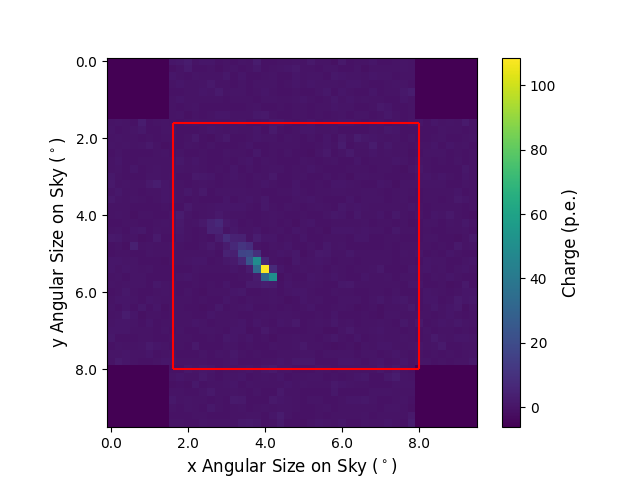
\includegraphics[width=0.7\textwidth]{figures/gammacut.png}
  \caption{A charge image from a simulated $\gamma$-ray event from the point source run dataset as described in section \ref{Datasets}. The region that survives the geometry cut is highlighted in red, the holes in the camera geometry to accommodate the flasher calibration system can be seen in the corners.}
  \label{fig:gammacut}
\end{figure}

\begin{figure}
  \centering
  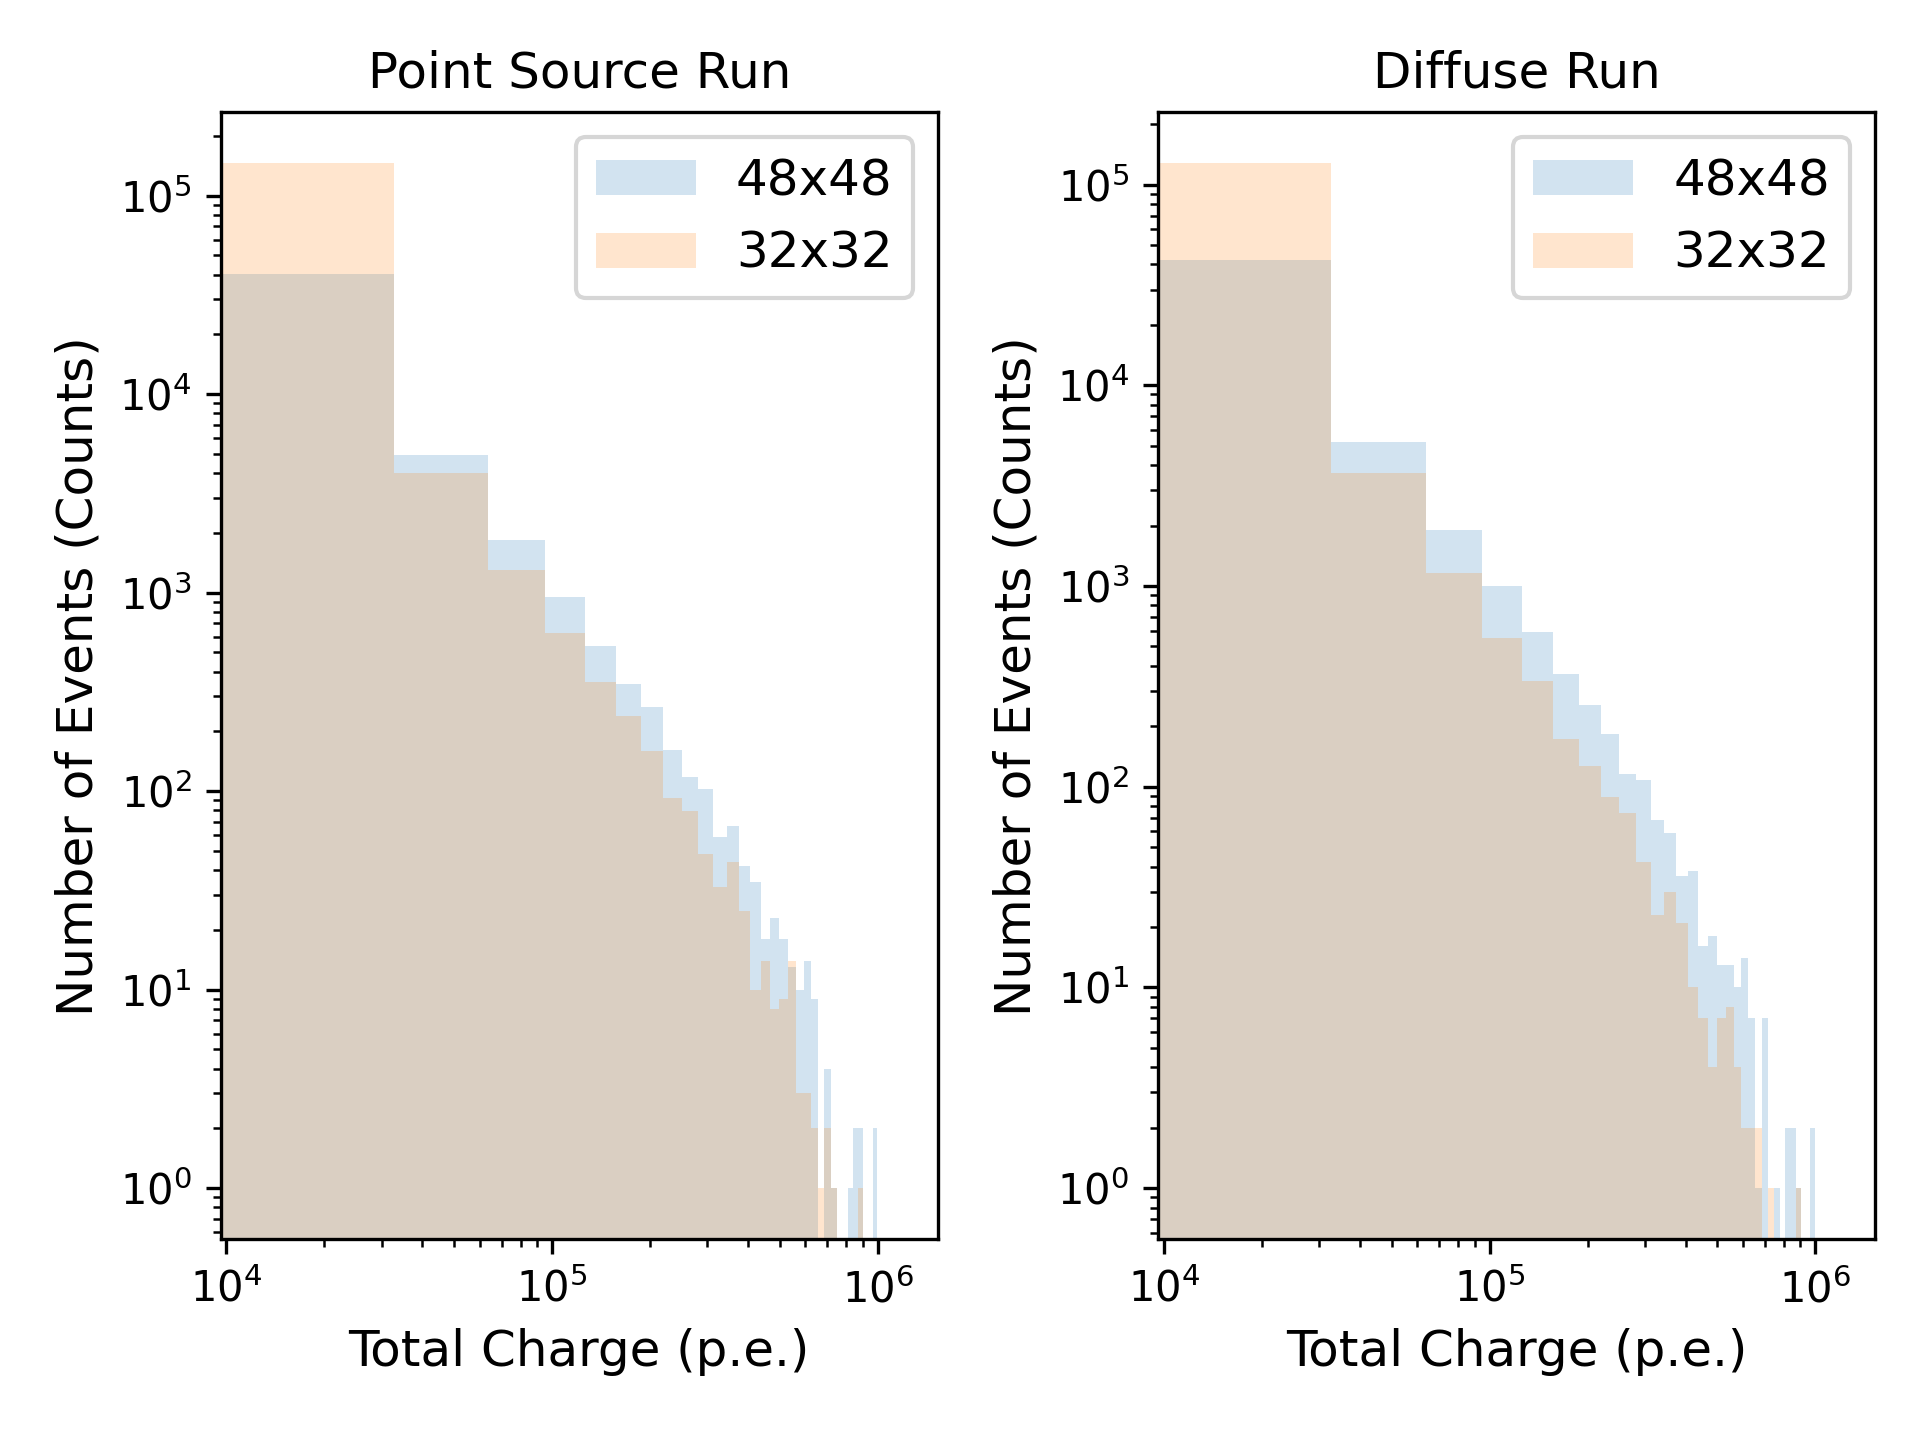
\includegraphics[width=0.7
  \textwidth]{figures/chargehistlog.png}
  \caption{Total integrated charge from all four telescopes over the two datasets used, as described in section \ref{Datasets}. Comparisons between the complete camera (48x48) and the cropped central region (32x32) are shown.  Most of the charge losses appear to be Night Sky Background photons as the two distributions are smooth and close together. The same logarithmic binning is used for both the cropped and uncropped regions.}
  \label{fig:chargehist}
\end{figure}

\subsection{Analysis Pipeline}
In order to perform our analysis, we used the \textit{Keras}  \cite{Keras} deep learning Python package with the \textit{Tensorflow\_gpu} backend \cite{tensorflow}. We also used the \textit{scikit-learn} \cite{scikit} and \textit{matplotlib}  \cite{matplotlib} packages to analyse and plot the results. The analysis pipeline we developed to perform this is illustrated in Figure \ref{fig:wavelearn}. Similarly to \cite{Shilon}, we use a mixture of convolutional layers and recurrence (specifically ConvLSTM2D layers, algorithmic details of which can be found in \cite{shi}) to robustly handle data from multiple telescopes. We compared four different techniques (Methods A-D) for classifying events on a like for like basis with these networks. These are summarised in Table \ref{table:methods} and detailed in the next three paragraphs. 

\begin{table}[ht]
    \centering
    \resizebox{\textwidth}{!}{
    \begin{tabular}{c|c|c|c}
    \textbf{Method} &\textbf{Pixel Maps Used} & \textbf{Ordering} & \textbf{Parameters}\\
    \hline
    A& Timing& Median Peak Time & 293,673\\
    B& Charge, Timing, Mean Amplitude, Peak Amplitude & Median Peak Time & 301,233\\ &FWHM, RMS, RT, FT& \\
    C& Charge & Size Parameter & 293,673\\
    D& Charge & Median Peak Time & 293,673\\
    \end{tabular}
    }
    \caption{Summary of methods used. The ordering of input channels into the ConvLSTM2D networks is as presented in this table. The number of trainable parameters is also shown, highlighting the effect of using a different number of channels in method B.}
    \label{table:methods}
\end{table}
\subsection{CHEC Camera Geometry}
Part of the challenge in the Shilon et al. work \cite{Shilon} was developing an unbiased method to handle Cherenkov camera images that are from a non-square (typically hexagonal) pixel grid \cite{Hexagdly}.  CHEC has largely square pixel geometry, bar for holes in its corners to accommodate the flasher calibration system. In our work, in order to be conservative and minimise the risk of potential geometric bias in which event classifications might be affected by proximity to these corners (which could be the case if they were instead filled by constant values), we simply crop images to the central region of the camera. This can be seen in Figure \ref{fig:gammacut}. This is unlikely to have a serious effect on the signal from the EAS as our simulation set-up (described in Section \ref{Datasets}) produces images where the shower is close to the centre of the camera (as shown in Figure \ref{fig:chargehist}). We disregard the small amounts of `dead space' between CHEC photomultiplier blocks for the same reason. More advanced tools are currently under development to cope with these issues \cite{dl1dh} \cite{thomas}.

\subsection{Experimental Methods}
In this subsection, we detail the four analysis methods we explore. For method A, we use the available waveform information to generate a 2D timing pixel map across the camera plane. We then select the pixels that have a large waveform amplitude, and set the other pixels in the pixel map to zero, in order to highlight the position of the shower in the image. The location of the peaks themselves is found using a wavelet convolution of width 8 and the \textit{scipy} \textit{signal.find\_peaks\_cwt} function \cite{scipy} \cite{findpeaks}. These four timing pixel maps (one for each telescope) are then fed into the network without anything else, in the order of increasing median photon arrival time.

In method B, we feed in the integrated charge image (without pixel selection) as the first channel to the ConvLSTM2D. We then feed in the timing pixel map created using the same technique as method A as the second channel, and similarly cut 2D pixel maps of six other parameters from the smoothed waveform: the mean amplitude, the peak amplitude, the root mean square value (RMS), the full width at half maximum (FWHM, calculated using a B-spline interpolation \cite{scipy}), the pulse rise time (RT) and the pulse fall time (FT) relative to the peak of the waveform. Both the RT and FT are calculated using a change-in-gradient method. This results in four images each with eight channels being fed into the ConvLSTM2D; examples of these pixel maps are shown in Figure \ref{fig:wfplot}. These channels are treated as extra dimensions in the input tensor, as Red, Green and Blue channels would be for a colour image.

Method C uses only charge images, ordered such that those with the largest total charge appear first in the LSTM sequence (as in \cite{Shilon}). It should however be noted that we do not perform an exact replication of the method in \cite{Shilon}. This is due to a number of factors. Firstly, we consider different instruments with differing camera designs and operational energy ranges. Secondly, we use a marginally different ConvLSTM2D network architecture (due to the CRNN code from \cite{Shilon} being proprietary), this differs from the CRNN architecture in that recurrent (LSTM-like) features are included from input layer until the final layer of the network (though the basic principle of merging convolutional and recurrent features is the same). We also use differing hyperparameters, partially due to this different architecture, and partly because the differing plate scales and operational energy ranges of the H.E.S.S.-1 cameras and CHEC means that there is no guarantee that the ideal hyperparameter choice will be the same for both instruments. This hyperparameter choice can have a significant effect in CNN-based analysis \cite{hyperopt}. Finally, in order to test the efficacy of CNN-based background rejection against electrons, we include these (realistically) in the analysis whereas \cite{Shilon} did not. This would cause differences with the training of any machine learning classifier (particularly in the diffuse case) as there are two nearly identical data samples with differing class assignments.

\begin{figure}[ht]
  \centering
  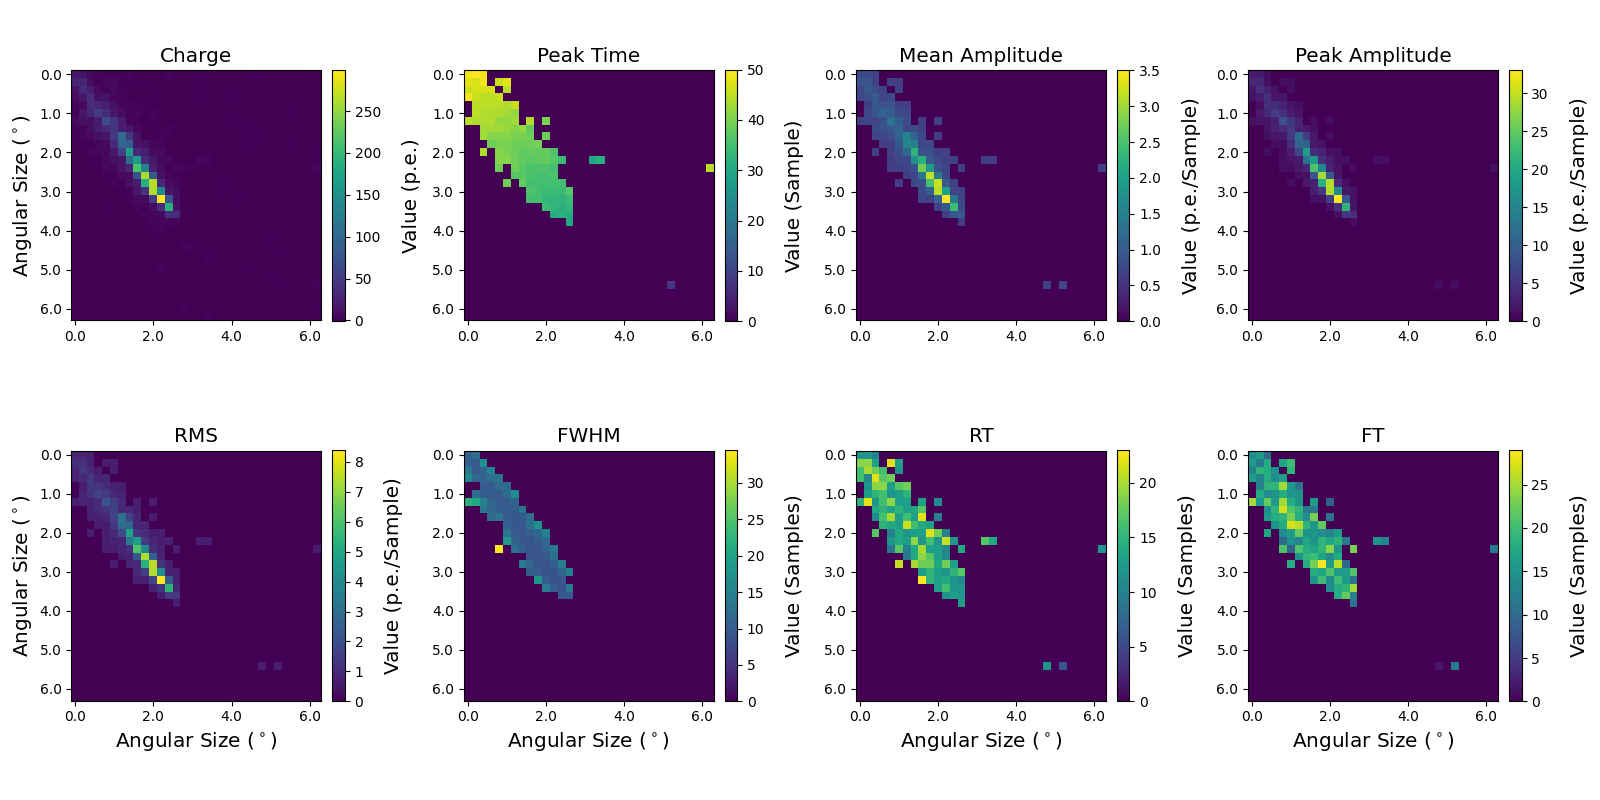
\includegraphics[width=\textwidth]{figures/56tgamma.png}
  \caption{As an illustration of the different pixel maps used with Method A, this figure shows pixel maps used (cut to the central region of the camera) from a $\mathrm{56\,TeV}$ $\gamma$-ray event in the point source dataset for one telescope. Note that these pixel maps are normalised prior to analysis, and that 1 sample represents approximately 1ns.}
  \label{fig:wfplot}
\end{figure}
In method D, we extract the median photon peak time from the waveforms and use this as a time proxy to order the images in place of the sum of the photomultiplier charges (as used in method C). In this case the only images actually fed to the network are those of integrated charge. As such the only difference between methods C and D is the order in which the charge images for an event are fed into the ConvLSTM2D, such that we can test what effect this has. Therefore methods A, C and D all result in 4 images each with 1 channel (i.e. grayscale) being fed into the ConvLSTM2D network.

\subsection{Hyperparameter Selection}
The datasets used, along with all training hyperparameters (see Table \ref{table:hyperparams}), were the same across all the four methods during the initial training. As this is intended as a differential study, we did not perform hyperparameter optimisation. Whilst there are Bayesian methods such as hyperopt \cite{hyperopt} for performing hyperparameter optimisation with CNN-based classifiers, it would not be trivial to cross-optimise the networks fairly across the four methods described here and it would also involve significant computational cost. Optimising the networks for say method B might disadvantage Method A unfairly. The least biased option is to use default hyperparameter options across the four methods. The ConvLSTM2D network architecture was also identical across the four methods, with the exception of the number of channels in the input vector (1-8).  This architecture is shown in Figure \ref{fig:model}.

\begin{table}[ht]
    \centering
    \resizebox{0.7\textwidth}{!}{
    \begin{tabular}{c|c}
    \textbf{Hyperparameter} & \textbf{Value}\\
    \hline
    Batch Size & 50 \\
    Training Epochs & 30 \\
    Training Optimiser & Adadelta \cite{adadelta} \\
    Adadelta Learning Rate & 1.0\\
    Adadelta Decay Factor &0.95 \\
    Output Layer Activation Function & Softmax\\
    \end{tabular}  
    }
    \caption{Training hyperparameters used; these were the same throughout all the networks during the initial training for both the point source and diffuse cases. The diffuse ES runs also used these hyperparameters.}
    \label{table:hyperparams}
\end{table}

\begin{figure}
  \centering
  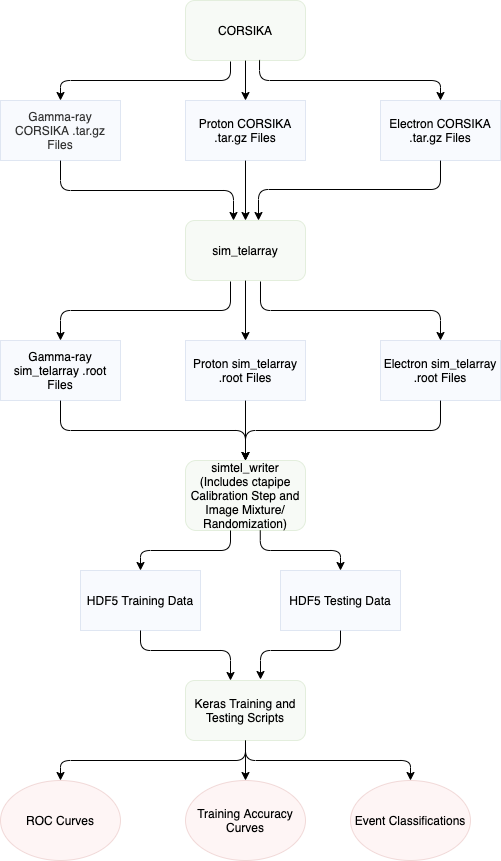
\includegraphics[width=0.7
  \textwidth]{figures/waveformstructure.png}
  \caption{The analysis pipeline used to generate the results in this paper. Ellipses denote analysis products, cornered rectangles denote stored files and rounded rectangles denote code elements.
  }
  \label{fig:wavelearn}
\end{figure}

\begin{figure}
  \centering
  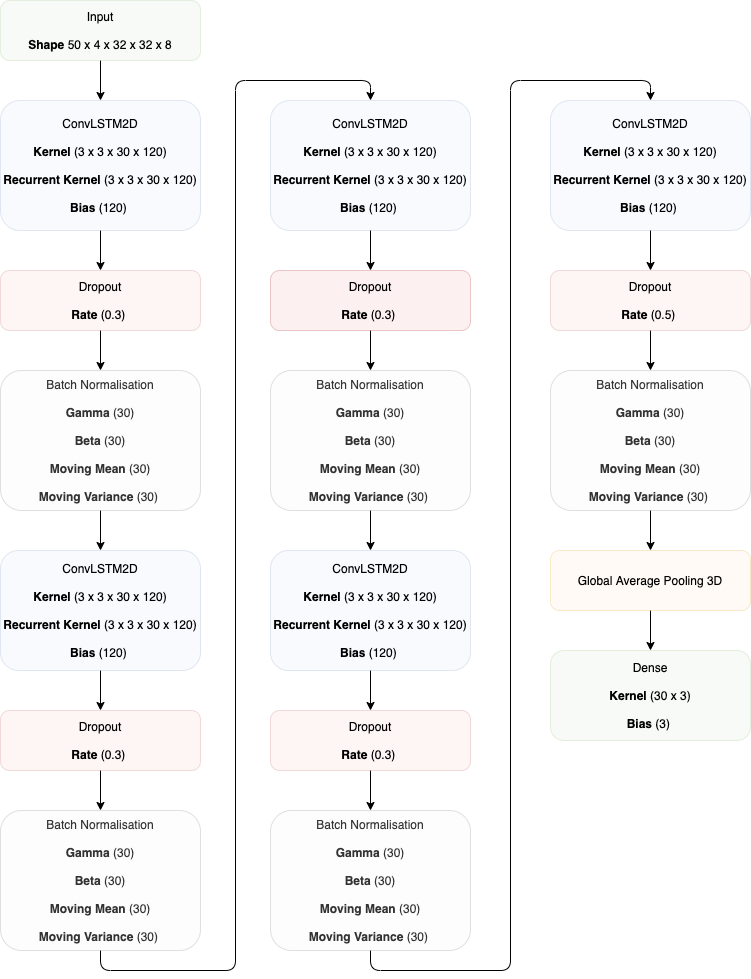
\includegraphics[width=0.9\textwidth]{figures/Newfig3.png}
  \caption{Example of our CNN-based ConvLSTM2D architecture. The only difference between the various methods A-D was the shape of the input vector, as some methods used more pixel maps than others.
  }
  \label{fig:model}
\end{figure}
\subsection{Training}
In order to prevent over-fitting, the ConvLSTM2D layers are followed by dropout and batch normalisation layers, and recurrent L2 regularisation \cite{Keras} is employed on the first two ConvLSTM2D layers. At the end of the network, global average pooling is used to connect to a final dense output layer of size 3 with a softmax activation function. The network is trained for 30 epochs with a batch size of 50 events per step, where the images and pixel maps have amplitudes normalised to the range [0,1]. There is a question over the efficacy of normalisation of IACT images with CNN-based methods as it can potentially prevent generalization, but in this case we observed superior overall training performance when the images were normalised.

\section{Results} \label{Results}
\subsection{Initial Results}
 The initial training took approximately 3 days on a NVidia 1080Ti GPU for each ConvLSTM2D network, meaning the training time for the results presented in Figures \ref{fig:trainlog}, \ref{fig:ROC} and \ref{fig:ROC2} was around a month. Each network for each method (A through D) and each of the two datasets (point source and diffuse) was trained from scratch independently, so each sub-figure in Figure \ref{fig:ROC} represents the test results for a uniquely trained classifier (the results from which are re\-plotted in Figure \ref{fig:ROC2}). We do not mix classifiers trained on different datasets, so classifiers trained on point source data are tested on (previously unseen) point source data, and not diffuse data. As such, and given the fact that there is no preferential direction in any of diffuse data \textit{CORSIKA}/\textit{sim\_telarray} events (as seen in Table \ref{table:Datasetparams}), the diffuse data results demonstrate classification power based solely upon shower morphology. Training accuracies as a function of epoch for this initial training are shown in Figure \ref{fig:trainlog}. This training was a significant computational task, and represents the limit of what can be performed with a single GPU. It should also be noted that in this particular use case, the `compute capacity' (NVidia's measure of a GPU's specifications) of the GPU is an important attribute due to the presence of RNN features in our network. Additionally, having a large amount of VRAM allowed for the processing of large datasets.
 
 \begin{figure}[t]
  \centering
  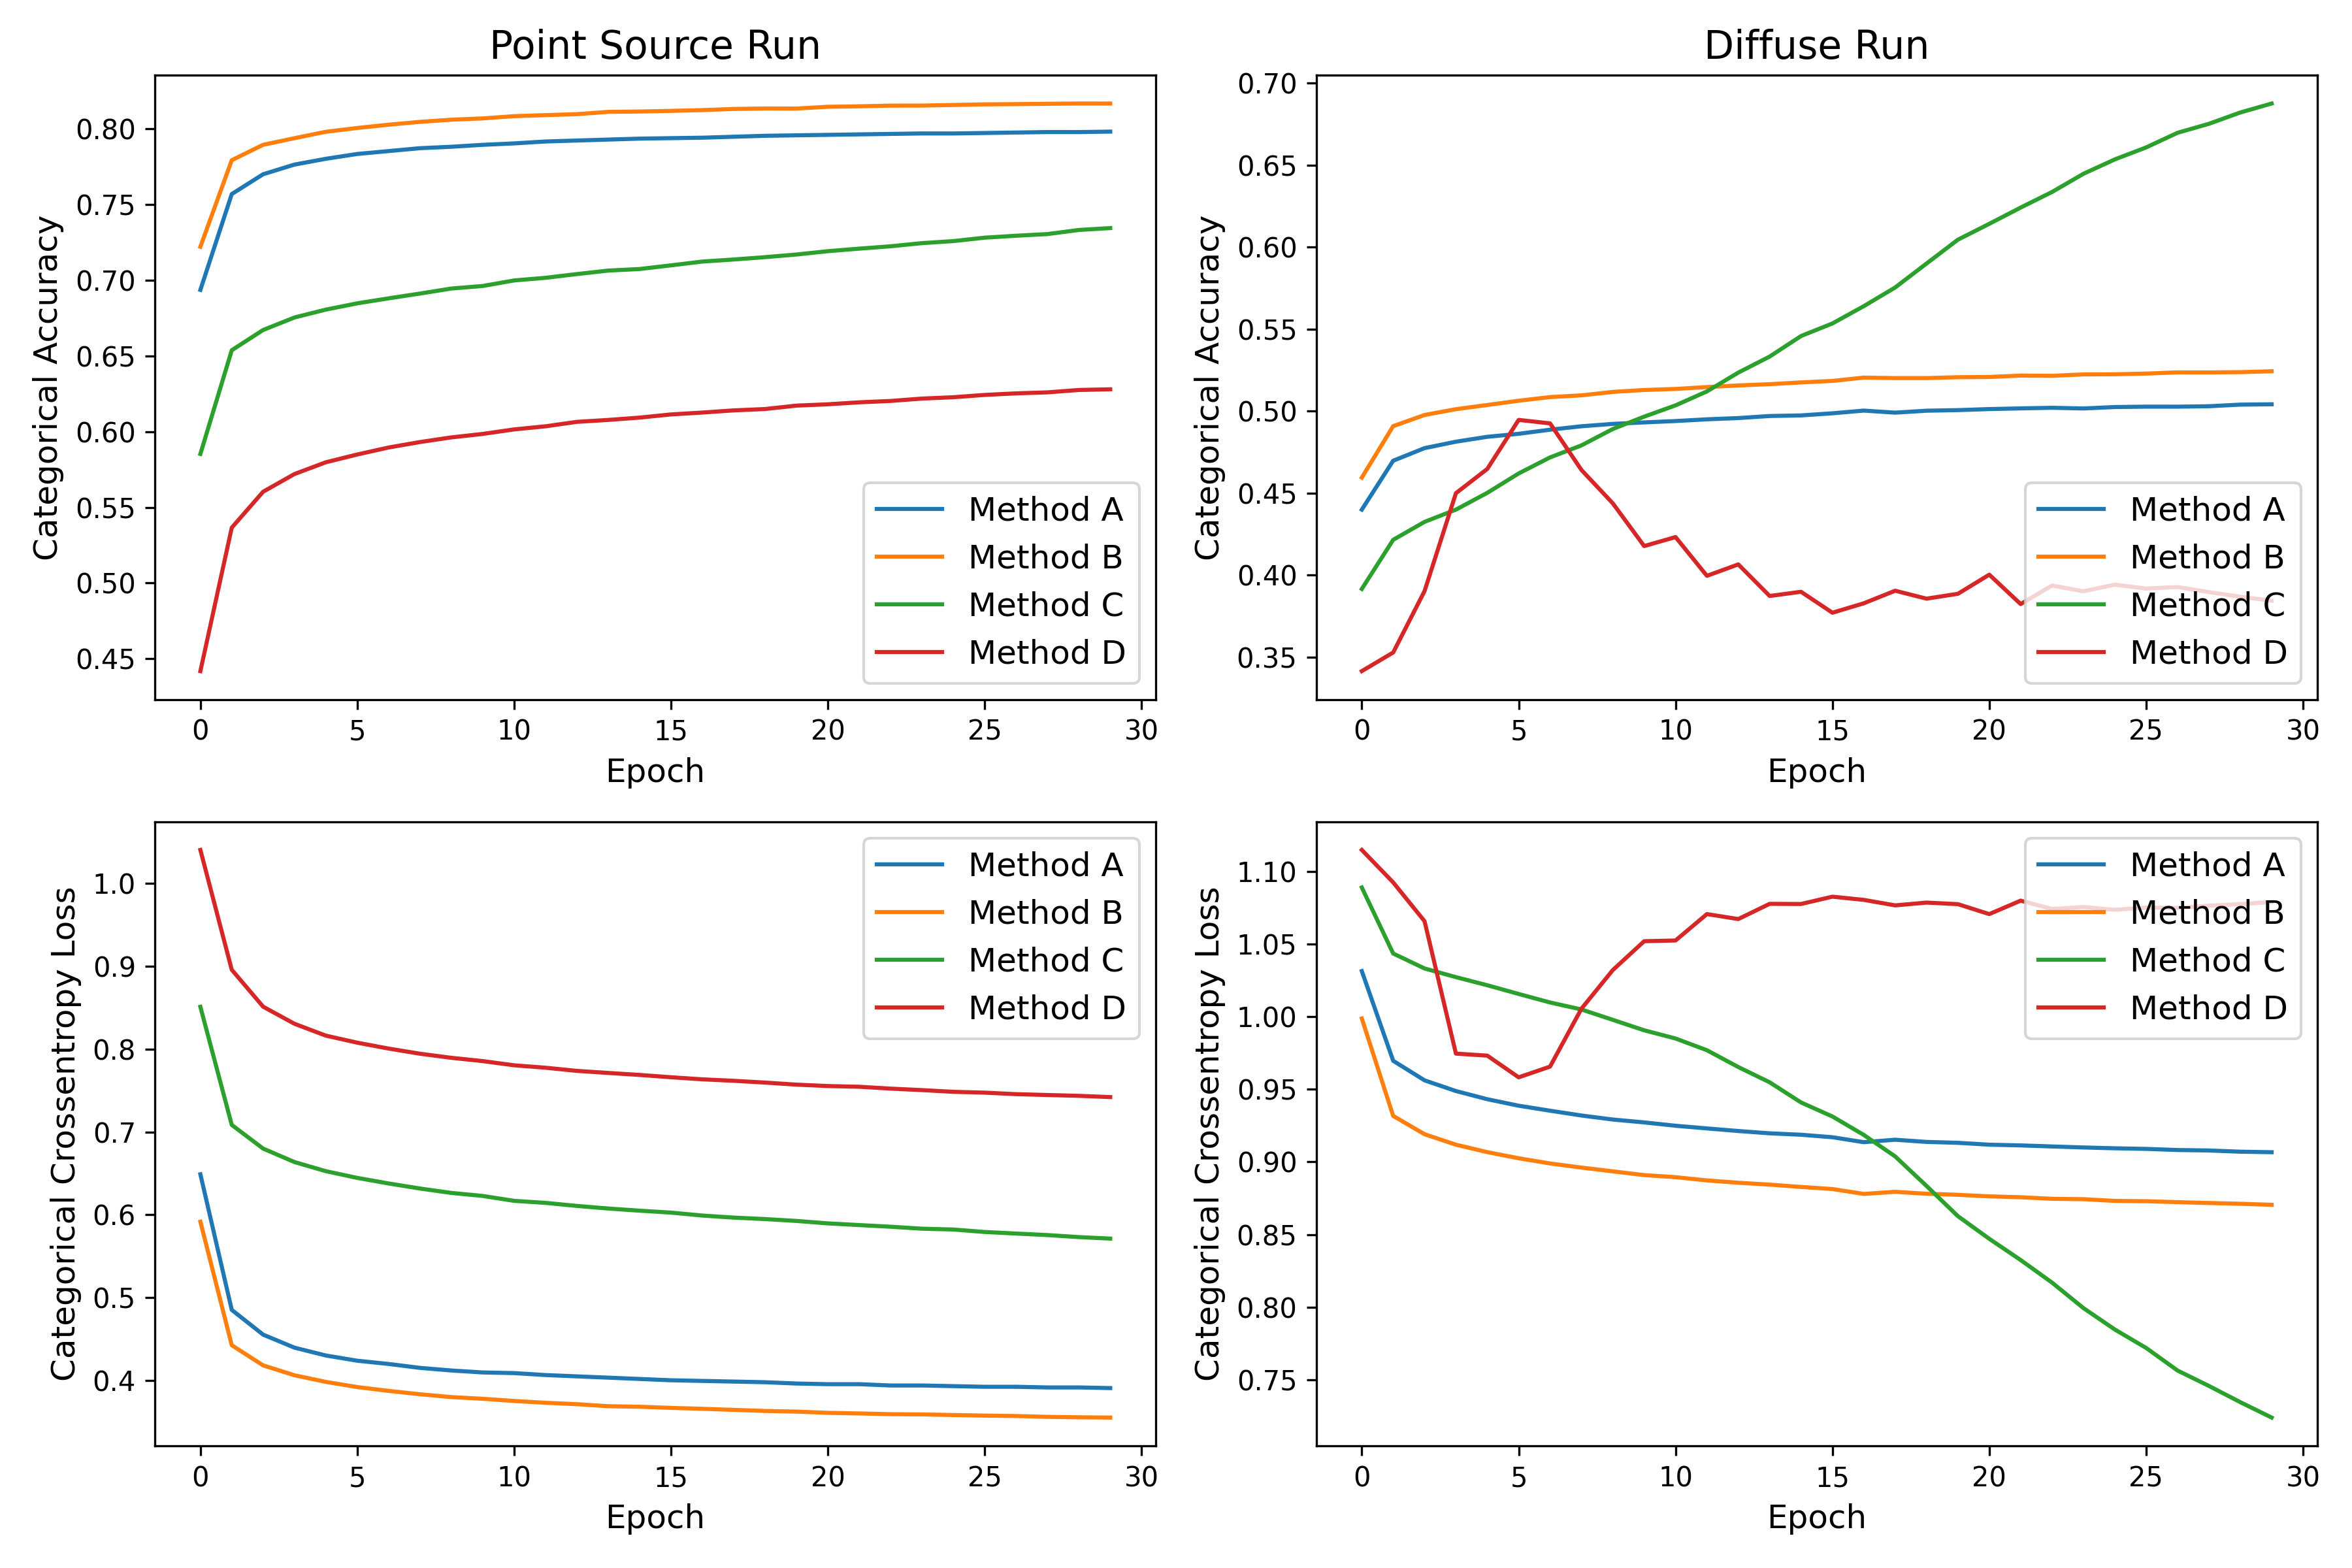
\includegraphics[width=\textwidth]{figures/trainlog.png}
  \caption{Initial training losses and accuracies for the four methods computed using the training dataset. Reasonable convergence is achieved for most methods given finite computational resources, but methods C and D in the diffuse case show some evidence of overtraining given their poor performance on the test data. This overtraining is evident here by either inversion or runaway acceleration in the loss function. It should also be noted that categorical accuracy and AUC values are not identically calculated metrics and the absolute values can differ.
  }
  \label{fig:trainlog}
\end{figure}
\begin{figure}
  \centering
  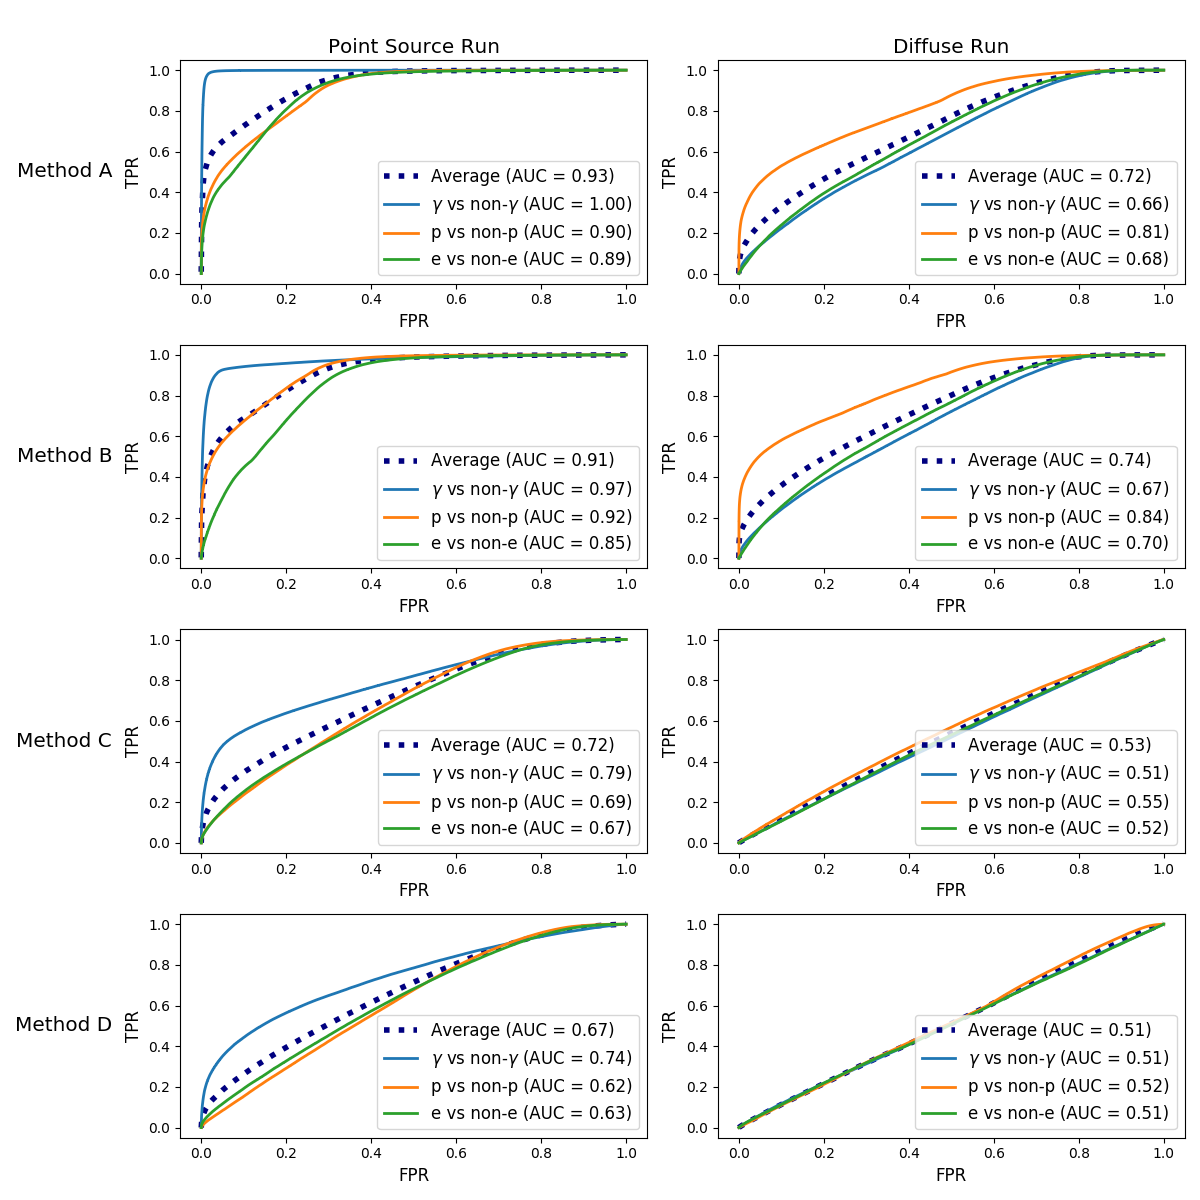
\includegraphics[width=\textwidth]{figures/final_newlabels.png}
  \caption{Receiver Operator Characteristic (ROC) curves for the four methods described showing the True Positive Rate (TPR) against the False Positive Rate (FPR). The Area Under Curve (AUC) performance metrics (the integral under these curves) are also shown. Deep learning analyses typically consider one versus all scenarios when calculating ROC curves \cite{scikit}, which is what we display here.  This means we consider if an event is classified a $\gamma$-ray or not a $\gamma$-ray when calculating the FPR and TPR in the multi-class scenario. Macro-averages across the three classes are also shown. It should be noted that the AUC results here and in Figure \ref{fig:ROC2} are only quoted to 2 decimal places and there are $\sim$700,000 testing events. As such, even in the optimal point source case, there are a number of misclassified events (i.e. $\sim$5500 $\gamma$-hadron misclassifications and $\sim$7000 $\gamma$-electron misclassifications for method A).
  }
  \label{fig:ROC}
\end{figure}
\begin{figure}
  \centering
  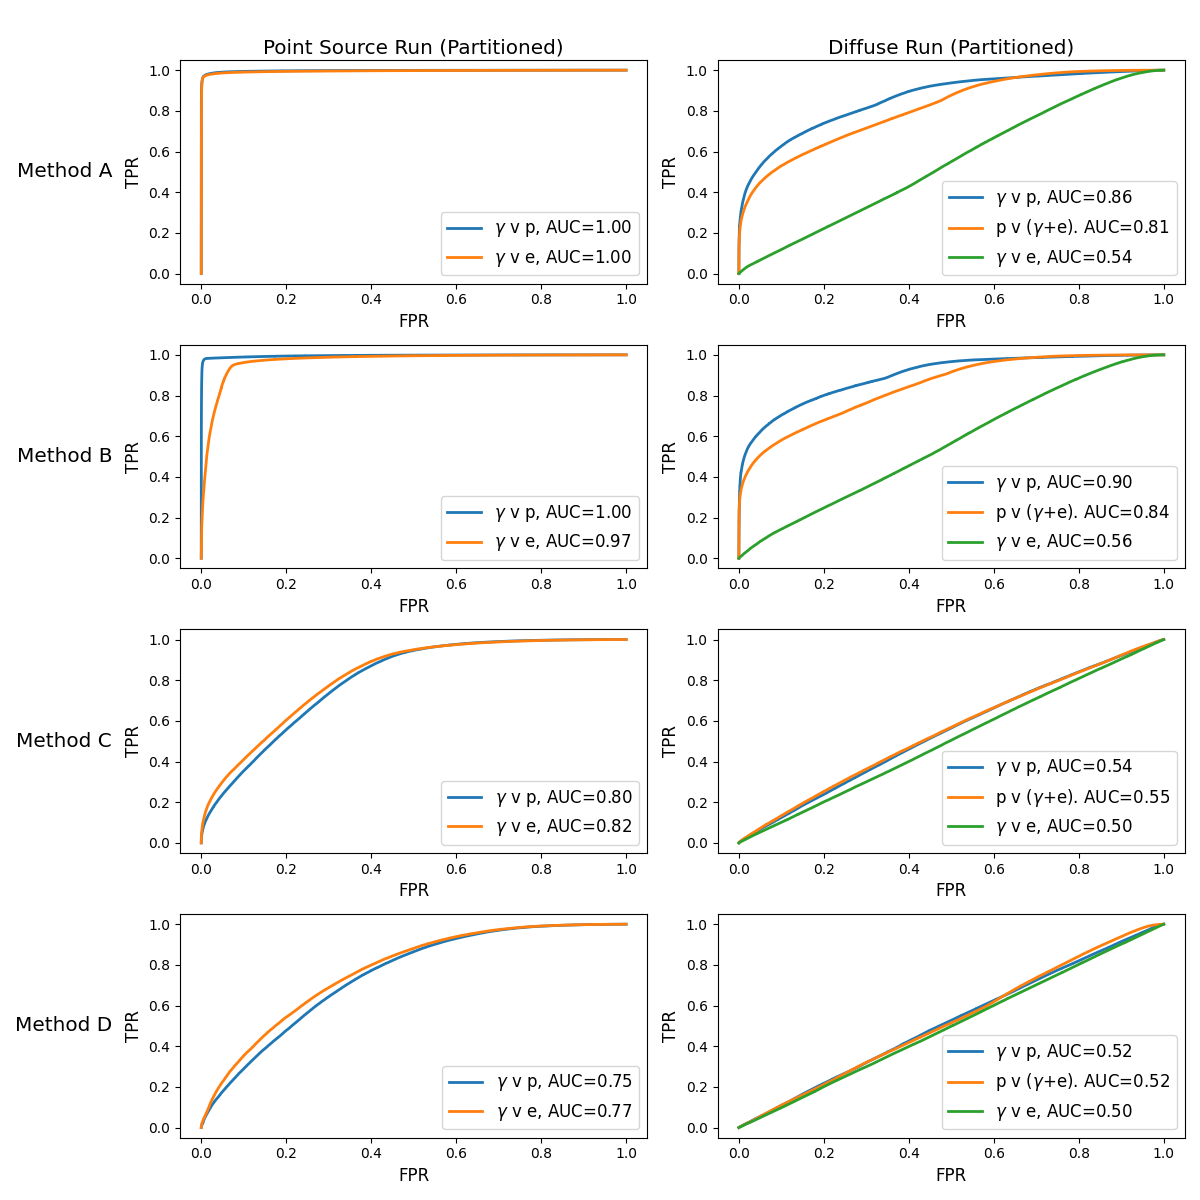
\includegraphics[width=\textwidth]{figures/abelardo.png}
  \caption{The same results from Figure \ref{fig:ROC}, this time shown in an astrophysical context. In this case we remove the other particle classifications from the analysis and consider only test FPR/TPR between various particles. In the point source run case, we consider the ROC curves for classification between $\gamma$-rays and protons and between $\gamma$-rays and electrons. This demonstrates the combined classification power of both morphological and directional information. The equivalent curves for the diffuse case highlight solely the morphological classification power. The proton versus ($\gamma$+e) curve demonstrates the difficulty  of distinguishing between $\gamma$-rays and electrons.
  }
  \label{fig:ROC2}
\end{figure}

\begin{table}[t]
    \centering
    \resizebox{\textwidth}{!}{
    \begin{tabular}{c|c|c}
    \textbf{Method} & \textbf{Point Source Run Classification Rate (Hz)}& \textbf{Diffuse Run Classification Rate (Hz)}\\
    \hline
    A & 308 & 296\\
    B & 240 & 231\\
    C & 339 & 320\\
    D & 308 & 336\\

    \end{tabular}  
    }
    \caption{Classification rates (the number of classifications per second) based on testing against $\sim$100,000 events for each method using 4 telescopes. Note that due to the LSTM features in our network this is substantially slower than classifications can be performed for Mono-telescope analysis ($\sim$1 kHz). This is also dependent on the GPU used (a NVidia 1080Ti in this case), and the data loader has not been fully optimised for speed. The test system had 32GB of Random Access Memory and operated at a clock speed of 1866 MHz.}
    \label{table:speed}
\end{table}
 \begin{figure}[t]
  \centering
  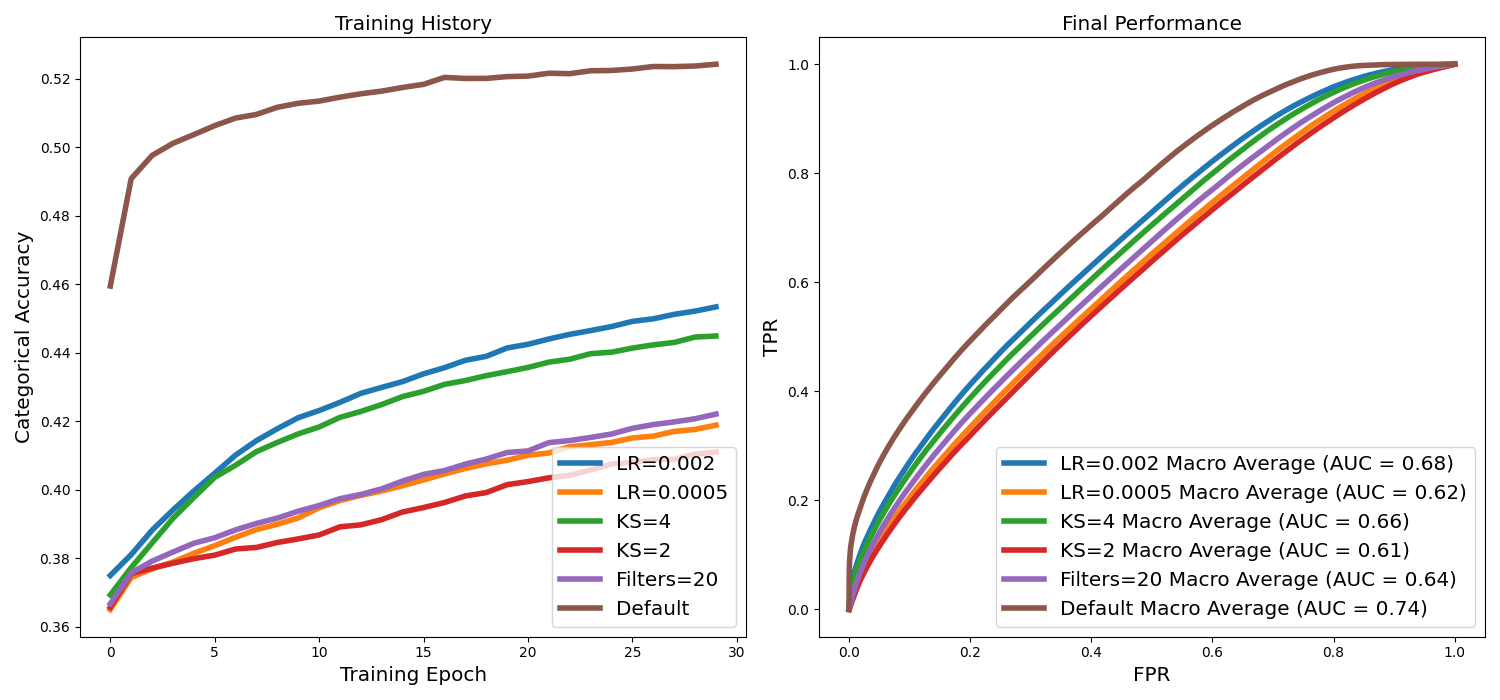
\includegraphics[width=\textwidth]{figures/modhyp.png}
  \caption{This plot shows the effect of modifying the hyperparameters for training Method B on the diffuse data. Left: The categorical accuracy as a function of epoch for the modified hyperparameter training runs. Right: The associated test ROC curves.
  }
  \label{fig:modhyp}
\end{figure}
\subsection{Difficulty in Identifying Classification Features}
Determining the source of classification power with ConvLSTM2D classifiers is non-trivial. Whilst gradient and perturbation based attribution techniques have been developed for standard single-image CNN classifiers (which can produce heat maps showing pixels relevant for classification) \cite{deepexplain}, open source packages for this do not currently extend support for such methods to the multiple image ConvLSTM2D case. As such, for stereoscopic analysis we are forced to interpret performance of these classifiers on different datasets in order to infer the information being used for classification. In our case, the results for the point source run and methods A and B achieve high performance metrics, but it appears as if this is as the classifier is largely using the directional information about the shower to perform classification, rather than morphological features in the images. This can be seen in Figures \ref{fig:ROC} and \ref{fig:ROC2}, as the classifier differentiates between $\gamma$-rays and other classes easily in the point source case for methods A and B, but not between the diffuse protons and electrons. But it is noteworthy that the ConvLSTM2D network performs this task so well and that methods A and B perform this in a superior way to methods C and D. This bodes well for future studies into directional reconstruction using CNN-based methods, as well as demonstrating the merit for multi-task deep learning studies that attempt to perform the tasks of event classification and directional reconstruction simultaneously (such as \cite{jacquemont}). This knowledge of the strong directional sensitivity of CNN-type methods can be used to inform the design of future CNN-based analysis pipelines for CTA.

In the diffuse case (where all three event classes come from an even spread of directions), methods C and D overtrain and cannot distinguish between any of the event classes. The timing based methods A and B appear able to perform good event classification based on shower morphology in Figure \ref{fig:ROC2} between the (combined) $\gamma$-ray and electron showers versus protons (that could be optimised further), but they cannot distinguish between the $\gamma$-ray and electron induced showers. The classification rates for the four different methods are shown in Table \ref{table:speed}, despite using many more pixel maps method B classifies at $\sim 70\%$ the rate of the other methods. Despite including more information than method A, method B doesn't appear to offer any significant improvement. This is likely as the timing information is likely to be the key component in the classification, though the marginally increased number of trainable parameters (as seen in Table \ref{table:methods}) for method B might disadvantage it slightly on a differential test basis.

\subsection{Effect of Hyperparameters}
In order to test the effect of varying hyperparameters, we ran additional training runs for Method B on the diffuse data. These runs were identical to the previous training runs for method B bar a single change each from the `default' hyperparameters shown in Table \ref{table:hyperparams} and Figure \ref{fig:model}. One run each had doubled and halved the Learning Rate (LR) from the default Adadelta value of 0.001, one run had all ConvLSTM2D kernel filter sizes (KS) set to 2x2, one with all filter sizes set to 4x4 and a final run with the number of filters per layer set to 20 rather than 30 (this value could not be increased due to VRAM constraints). The training accuracy curves (all showing reasonable convergence) and test results from this are shown in Figure \ref{fig:modhyp}. The `default' hyperparameter setup outperforms the alternatives, however this is to be expected as changing the \textit{Adadelta} optimiser parameters is not recommended by the developers of \textit{Keras} \cite{Keras}, and the 3x3 filter size option also provided the good results in the original ConvLSTM2D paper \cite{shi}. Whilst this gives us some idea of the spread in performance due to hyperparameter selection, this is not a substitute for an exhaustive hyperparameter space search, the optimal combinations of which are often not human-interpretable. The uncertainty associated with individual event classifications is also not trivial to obtain with CNN-type methods \cite{mike} \cite{gal2015}, and this is likely to be a necessary area of further development for these analysis techniques.

 \begin{figure}[t]
  \centering
  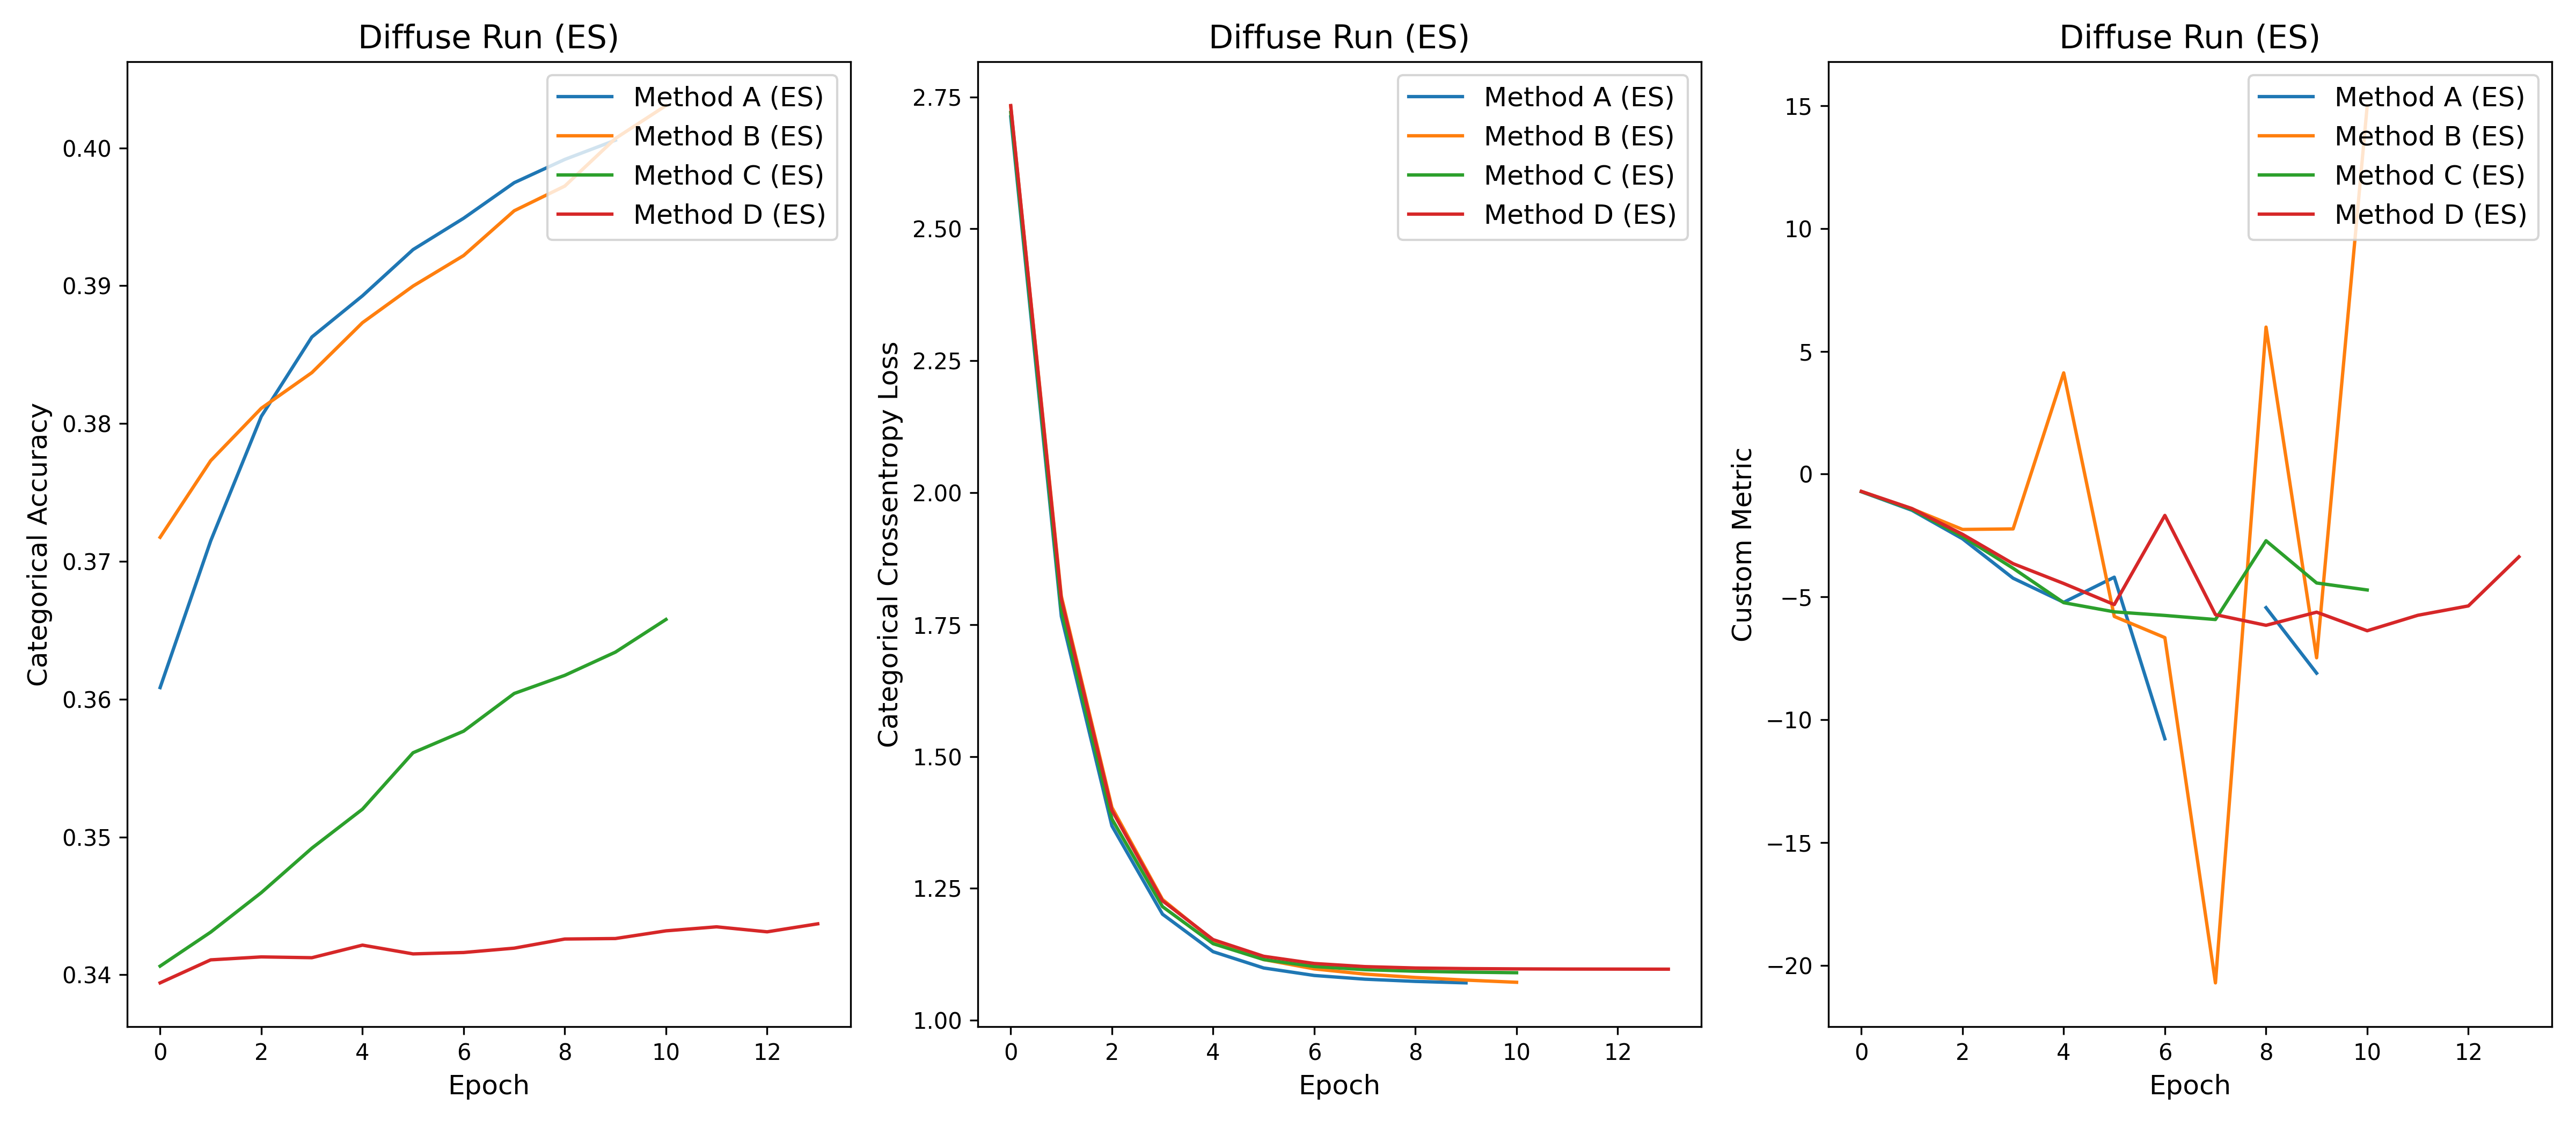
\includegraphics[width=\textwidth]{figures/trainlogES.png}
  \caption{Training total loss, categorical accuracy, and custom metric (M) values for the four ES runs, all on the diffuse data. The custom metric curve for method A diverges towards an infinite value due to finite numerical precision on epoch 7.
  }
  \label{fig:trainlogES}
\end{figure}

\subsection{Convergence and the Effect of Early Stopping}
\begin{figure}
  \centering
  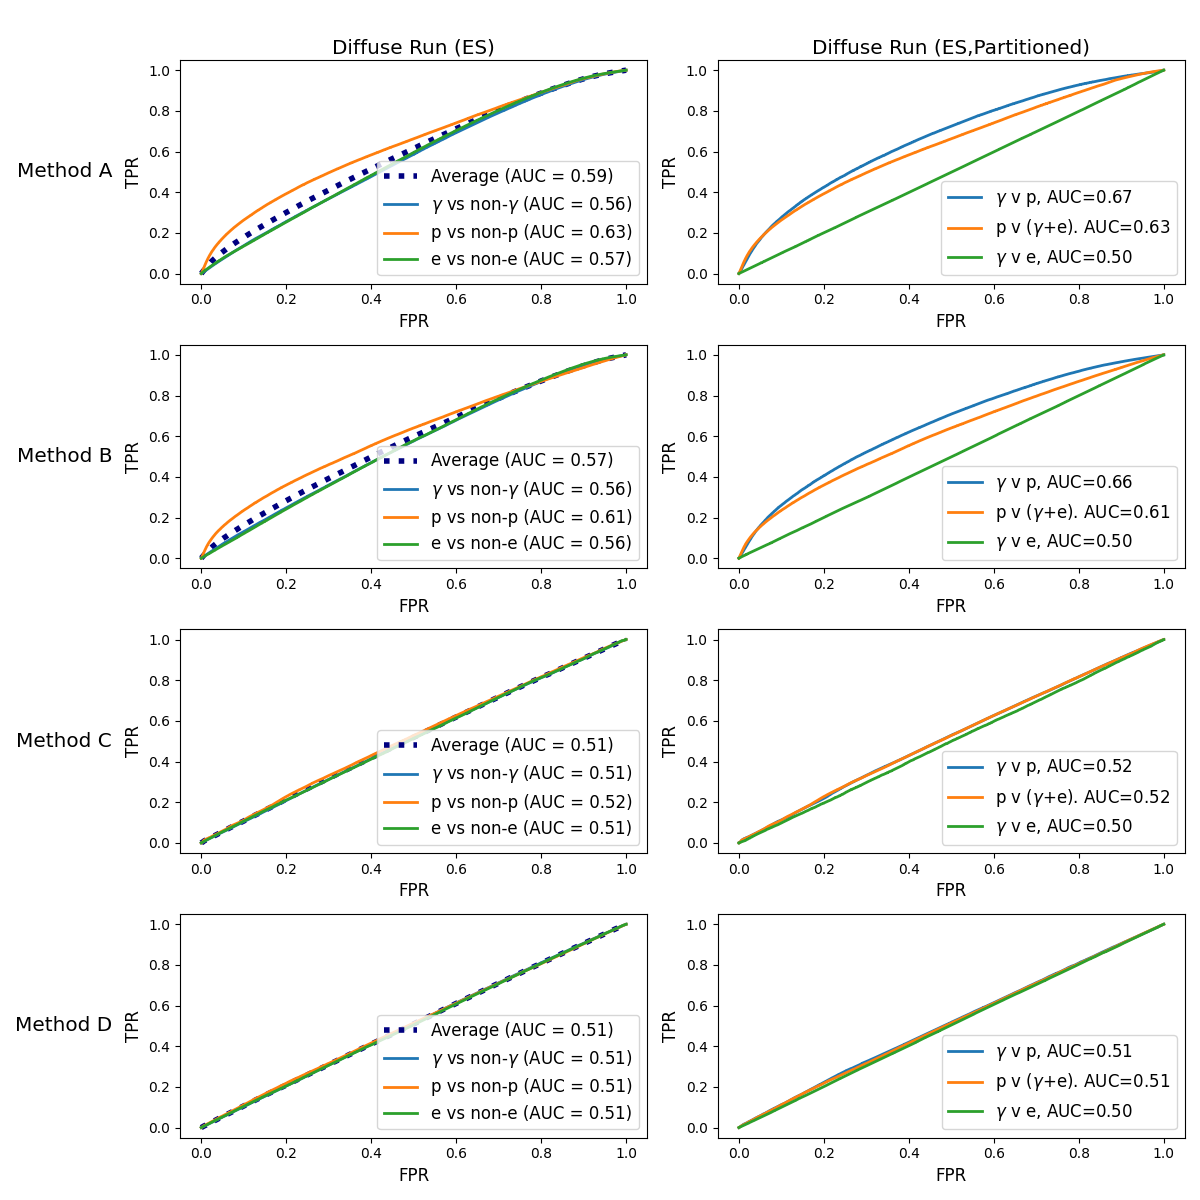
\includegraphics[width=\textwidth]{figures/esplot.png}
  \caption{This figure shows the final results from the ES runs, which are only trained and tested on diffuse data. Left: The results presented in the standard machine learning one versus all approach as in Figure \ref{fig:ROC}. Right: The same ES results shown in the astrophysical context of Figure \ref{fig:ROC2}.
  }
  \label{fig:ROC3}
\end{figure}

In order to investigate the influence of overtraining of methods C and D in the initial diffuse runs (as seen in Figure \ref{fig:trainlog}) with the original hyperparameter configuration from Table \ref{table:hyperparams} and Figure \ref{fig:model}, we ran additional training and testing runs on this diffuse data using this `default' configuration along with two early stopping criteria (that we reference by the abbreviation ES). Early stopping in \textit{Keras} allows for the stopping of training when there is an inversion in a chosen metric function, and for the restoration of the earlier optimal model weights obtained during training. In the case of preventing the overtraining scenario we observed for method D (where there's a clear inversion in the loss at epoch 6), the choice of this early stopping metric is the total loss function used during training. However, choosing such a metric to prevent the overtraining scenario we observed for Method C whereby there is undesired, runaway acceleration in the training data loss is more complex. As such, we implemented a custom second metric (M) of the form
\begin{equation}
    M=\frac{1}{0.7-0.8*L}
\end{equation}
where L is the total loss shown in for example Figure \ref{fig:trainlog}. This L includes both the categorical cross-entropy loss and the regularization penalties which we explicitly sum over the first two ConvLSTM2D layers. We intentionally designed this metric as it has a turning point (that will trigger the \textit{Keras} early stopping) around the epoch that method C appeared to start overtraining in the original training runs. For both metrics we choose a \textit{patience} parameter of 3, representing the number of epochs to tolerate the inversion of the metrics.

The training curves and results from these ES runs can be seen in Figures \ref{fig:trainlogES} and \ref{fig:ROC3}. During the ES training for Method A, the early stopping was triggered on epoch 10, for Method B and C on epoch 11, and Method D on epoch 14. We still observe superior performance (and some ability to perform gamma/hadron separation using morphological information) for the timing based methods A and B, despite this early stopping procedure (which was human-engineered for Method C). As such, we believe the superior performance of methods A and B in the diffuse case cannot be solely attributed to a bias from the non-convergence of the initial training for methods C and D, and is a result of the charge-only dataset used for methods C and D rather than an effect due to the design or optimisation of the classifier network.

The charge-only methods \cite{Shilon} (methods C and D) perform poorly in our analysis in both the point source and diffuse cases (regardless of whether early stopping is used or not); this isn't to say that such charge-only methods could not function well given additional hyperparameter optimisation and image cleaning. We seek simply to demonstrate the effectiveness of our timing techniques on a differential basis, which is confirmed by our results. As such, the absolute ROC, AUC, loss and accuracy values here should not be considered to be optimal for any of the four methods. It should also be noted that the realistic presence of electron events in the training datasets likely makes training the networks in the diffuse case significantly harder than straightforward $\gamma$-hadron separation given their similarity to $\gamma$-ray events, and this is likely part of the reason these two methods perform poorly in the diffuse case. Part of our reasoning behind these conclusions is that all four methods are affected to roughly the same extent ($\mathrm{\sim0.2\,AUC}$) by the change between (non-ES) diffuse and point source runs. Small variations in the accuracy values between the different methods could be statistical or due to hyperparameter configuration; averaging the results from multiple trials with different random seeds might help to confirm this, however this would be highly computationally intensive.

\section{Investigation into Identified Features}

\begin{figure}[ht]
        \centering 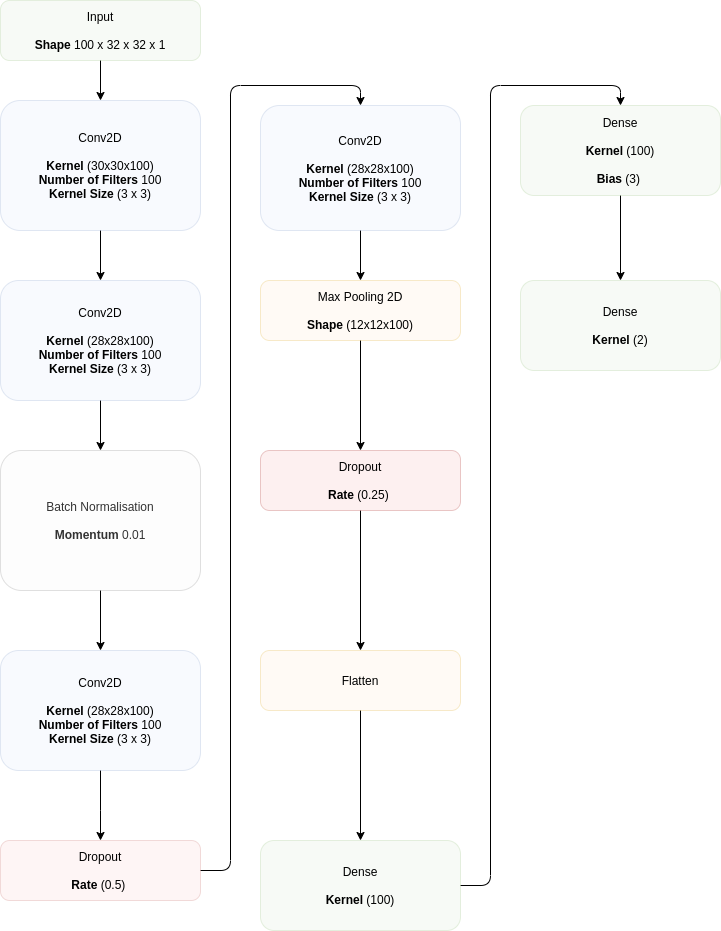
\includegraphics[width=0.8\columnwidth]{figures/newhyp.png}

        % read manual to see what [ht] means and for other possible options
        %\centering 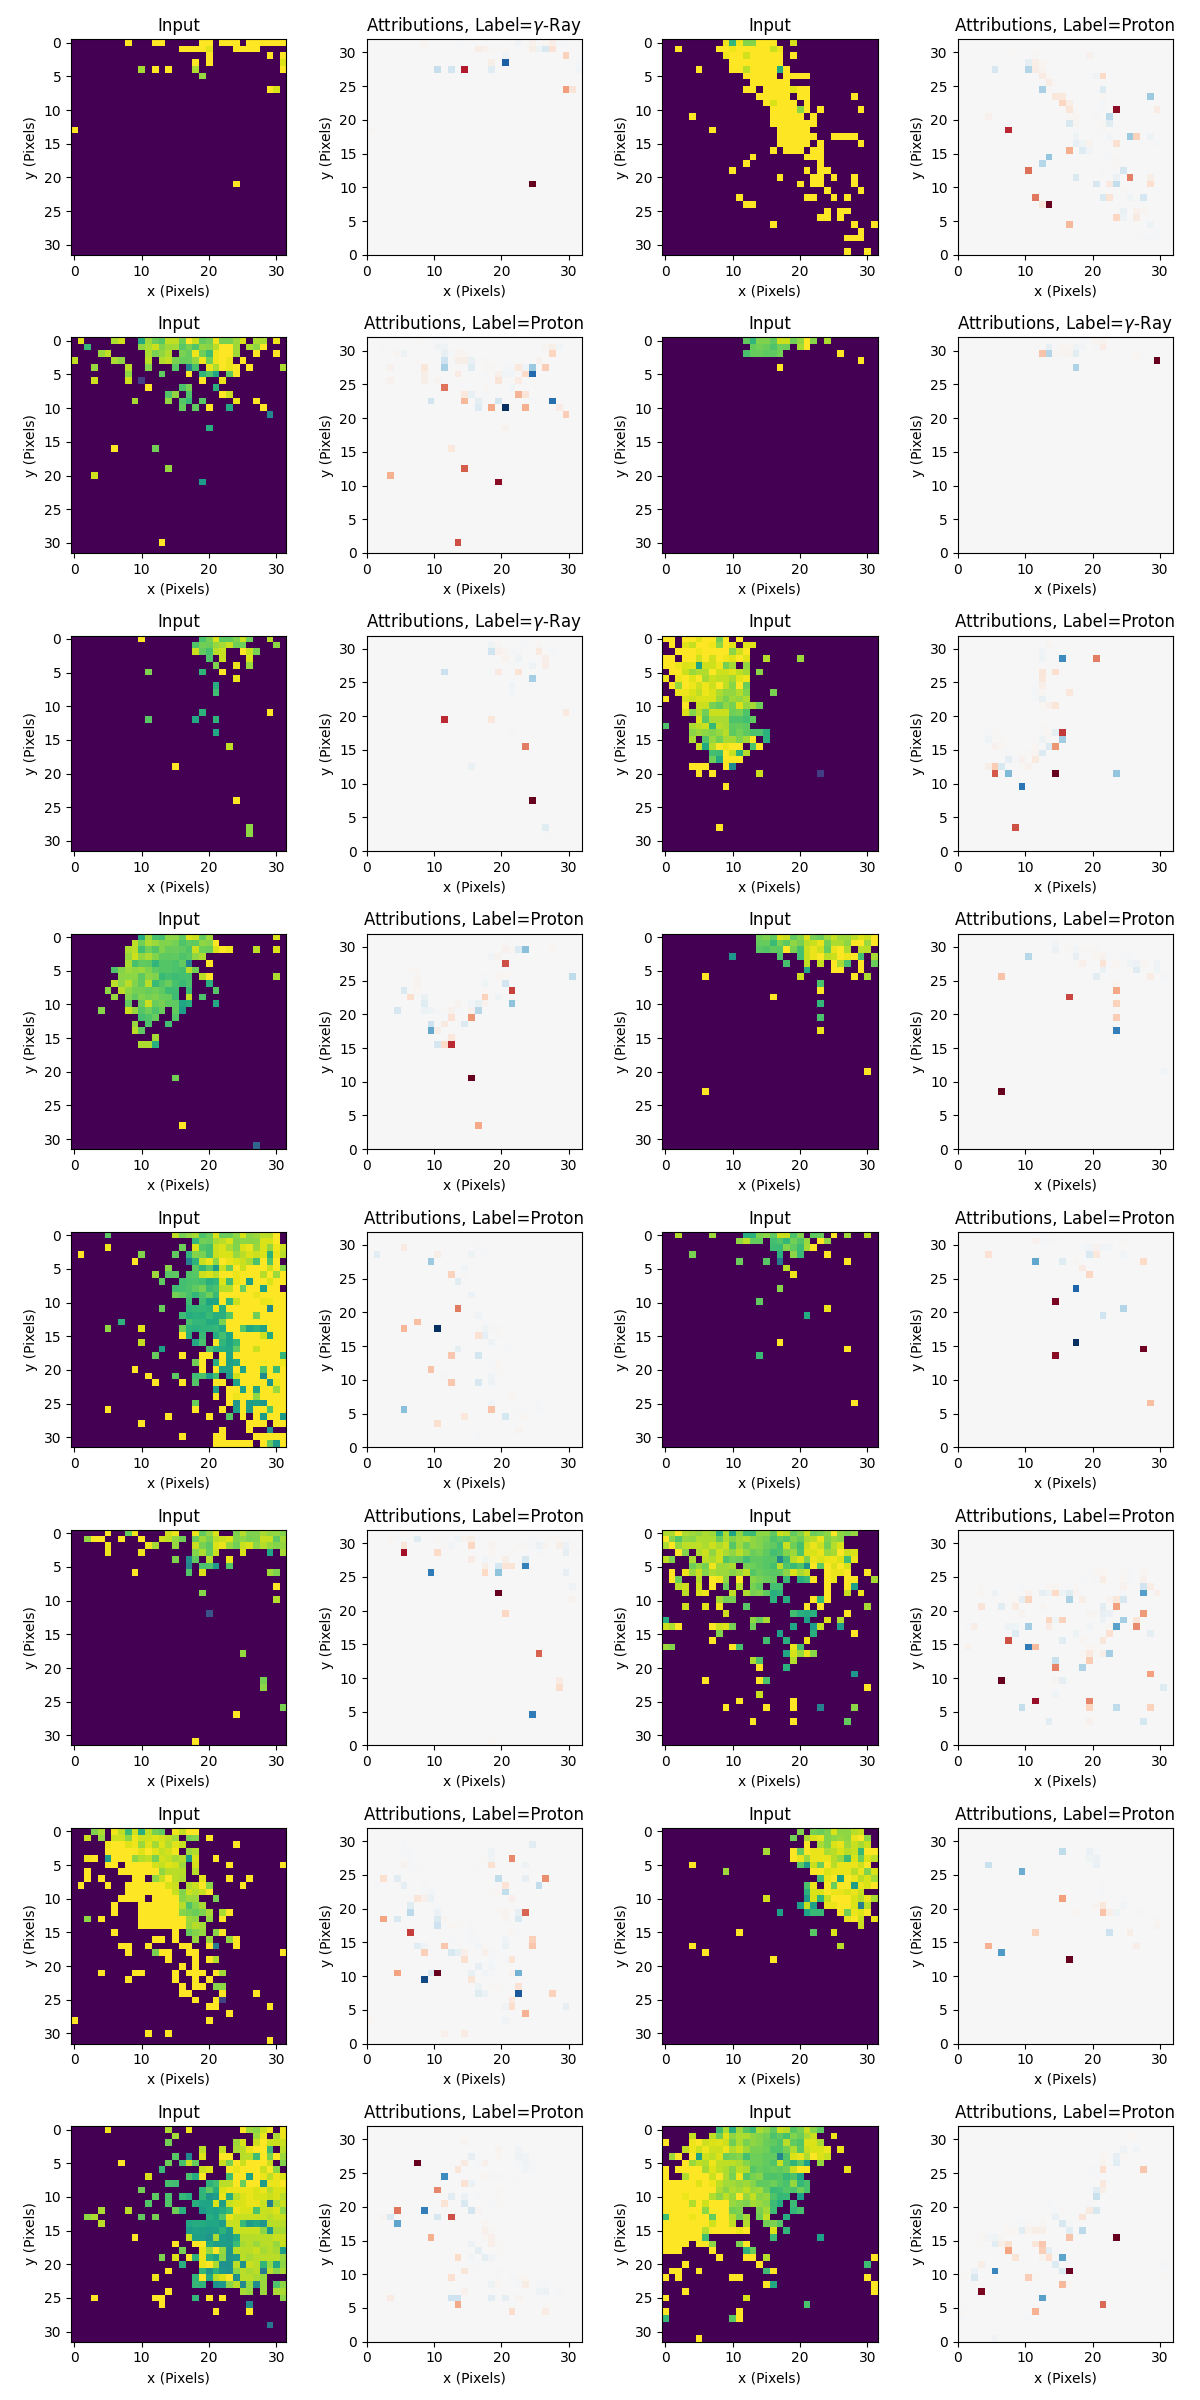
\includegraphics[width=1.0\columnwidth]{figures/newexpchec.png}

        % note that in above figure file name, "sr_setup",
        % the file extension is missing. LaTeX is smart enough to find
        % apropriate one (i.e. pdf, png, etc.)
        % You can add this extention yourself as it seen below
        % both notations are correct but above has more flexibility
        %\includegraphics[width=1.0\columnwidth]{sr_setup.pdf}
        \caption{
                \label{fig:lrparch} % spaces are big no-no withing labels
                % things like fig: are optional in the label but it helps
                % to orient yourself when you have multiple figures,
                % equations and tables
                The architecture of the single image CNN used for our LRP investigation. The architecture differed from that used for stereoscopic analysis by necessity,  both to achieve reasonable test accuracy and for compatibility with \textit{deepexplain}. 
        }
\end{figure}
\begin{figure}[ht] 
        % read manual to see what [ht] means and for other possible options
        \centering 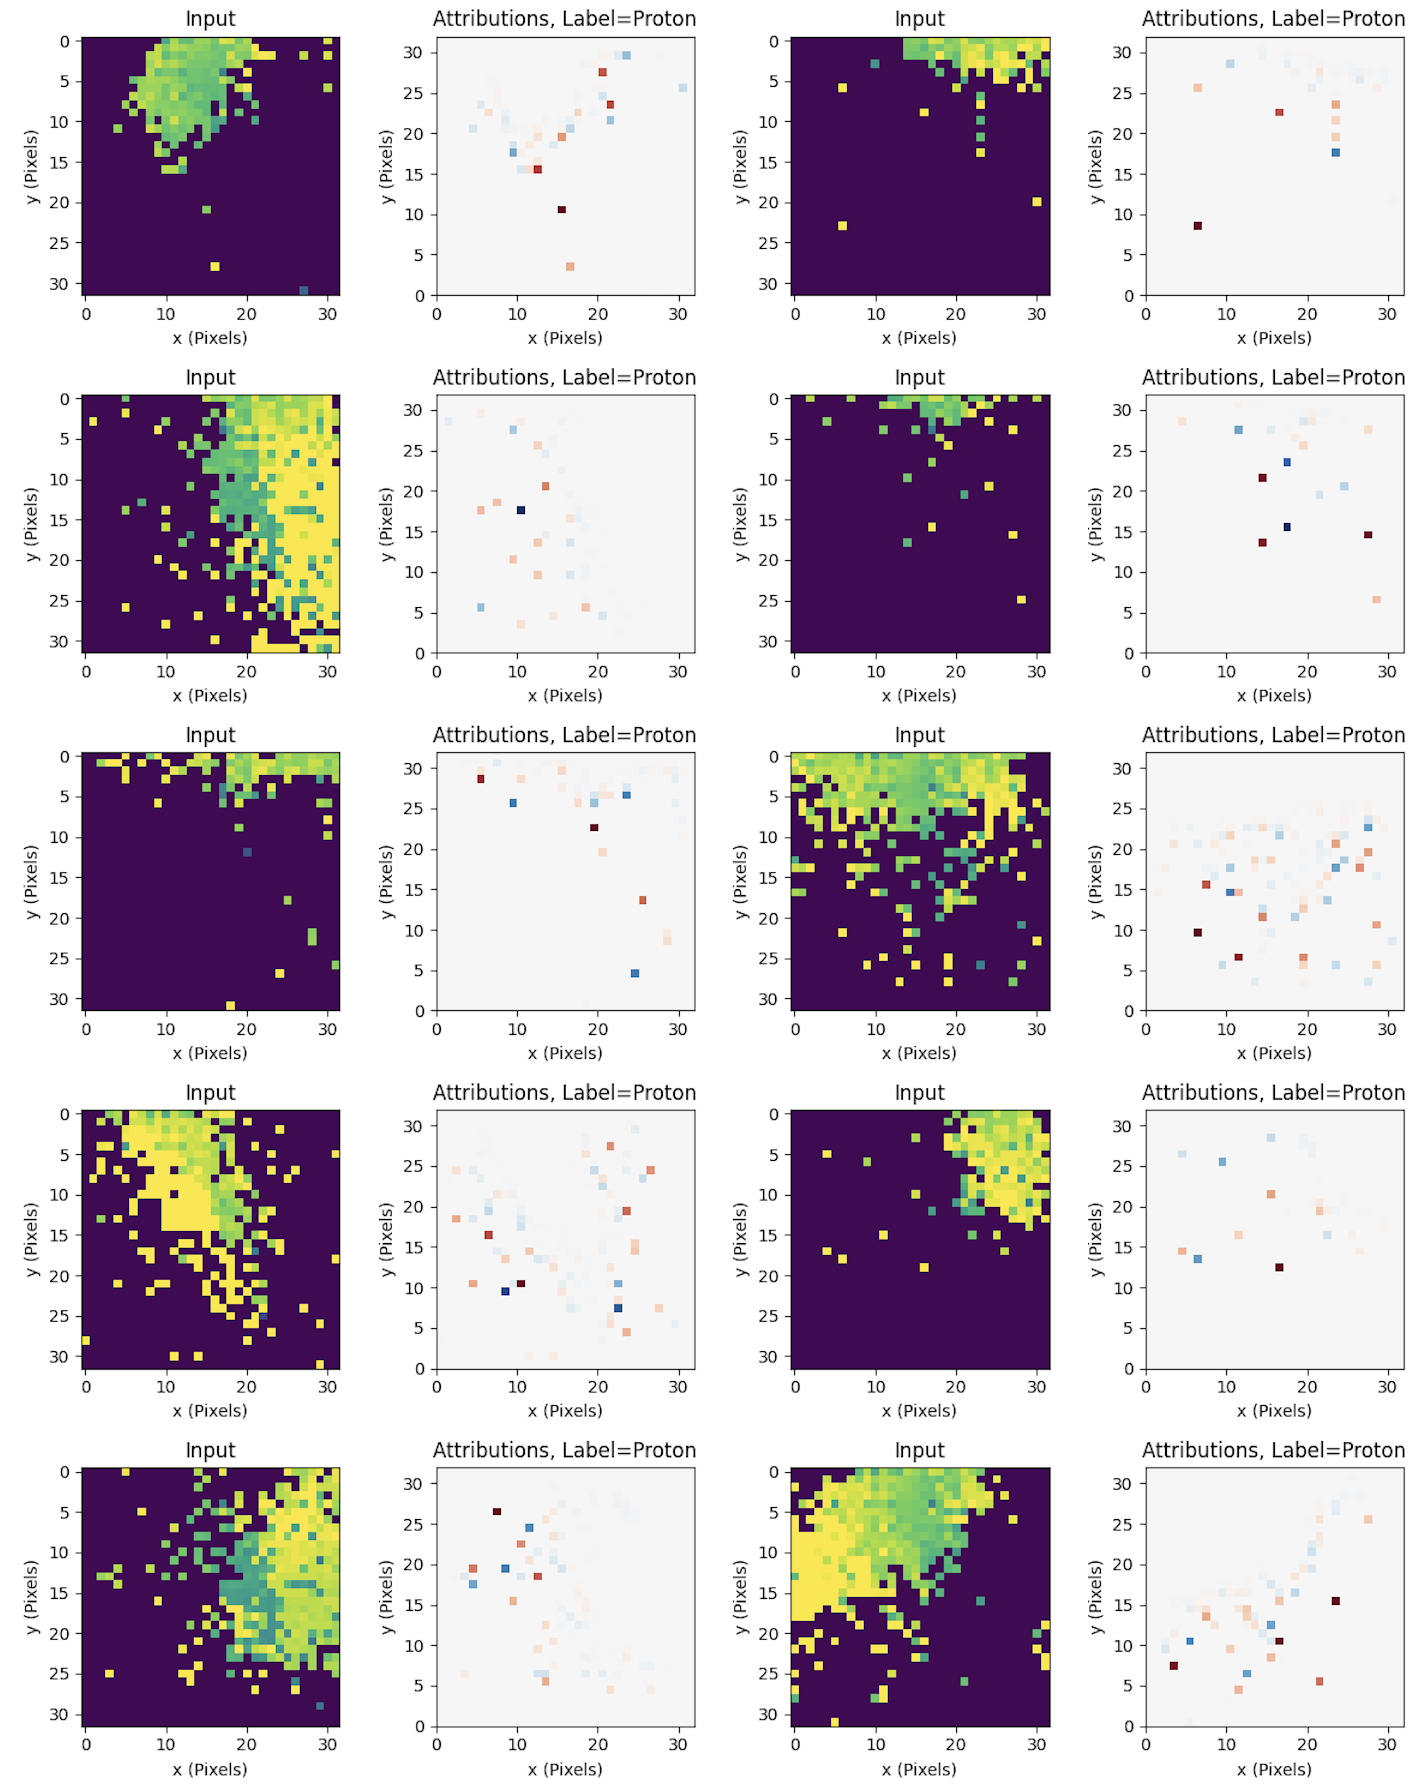
\includegraphics[width=1.0\columnwidth]{figures/newexpchec2.png}

        % note that in above figure file name, "sr_setup",
        % the file extension is missing. LaTeX is smart enough to find
        % apropriate one (i.e. pdf, png, etc.)
        % You can add this extention yourself as it seen below
        % both notations are correct but above has more flexibility
        %\includegraphics[width=1.0\columnwidth]{sr_setup.pdf}
        \caption{
                \label{fig:lrp} % spaces are big no-no withing labels
                % things like fig: are optional in the label but it helps
                % to orient yourself when you have multiple figures,
                % equations and tables
                The results of our LRP investigations. Test images fed to the network are shown along with the feature maps associated with them, where deeper shades of red indicate the pixels that contributed the most to the classification as a gamma ray induced shower or hadronic shower and deeper shades of blue pixels that counted against the classification.  
        }
\end{figure}
As mentioned earlier, whilst methods of feature identification do not exist for stereoscopic analysis, they do exist for single image classifier CNNs. Performing such analysis on single IACT images is worthwhile as it can demonstrate the capability of convolutional layers to extract physically meaningful features in IACT images. As such, we trained a single CNN classifier on single telescope timing histograms from the diffuse dataset (i.e. Method B), the architecture of which can be seen in Figure \ref{fig:lrparch}. As in the stereoscopic case, the images are cropped to the central region of the camera and are normalized, but the electrons are removed to ease training. In order to perform the feature importance analysis, this network had a different architecture to the ConvLSTM2Ds used earlier in this chapter. Additionally a cut on the size of the timing histograms was necessary to account for the fact that the simulation configuration necessary for multiple telescope analysis can produce a number of events with a low overall charge for given individual camera. Unfortunately this generated a greater than expected number of partially truncated events, which is not the case more widely in the dataset (as can be seen in Figure \ref{fig:chargehist}). There are two primary established techniques for performing this feature extraction \cite{deepexplain}; the first is to iteratively mask out features in input images and observe the change in CNN predictions (so-called occlusion methods). The second is to perform a weighted sum backwards through the network and identify the pixels that contributed most to a classification (so-called gradient based methods). We focus on the latter as it allows for pixels which counted against the classification to also be identified. Specifically in our case using the Layerwise Relevance Propagation (LRP) technique \cite{LRP}. This assigns a relevance to every $i$th neuron in layer $l$ in the network
\begin{equation}
r^{(l)}_i=\sum_j\frac{z_ji}{\sum_{i'}(z_{ji'}+b_j)+\epsilon\cdot\rm{sign}(\sum_{i'}(z_{ji'}+b_j))}r_j^{(l+1)}
\end{equation}
where $z_{ji}=w_{ji}^{(l+1,l)}x_i^{(l)}$, $w_{ji}$ is the weight associated with the $ji$th connection in the neuron, $x_i$ is an element of the input vector to a neuron, $b_j$ is a bias term and $\epsilon$ is a small term added to improve numerical stability. The ultimate values we want are the relevances for the input layer $r_i^{(1)}$. We used the \textit{deepexplain} package to perform this calculation.

The results from this investigation are show in Figure \ref{fig:lrp}, the classifier achieved a 70$\%$ test accuracy (likely a result of the training dataset not being designed for mono-instrument analysis). It appears that the position of the shower in the image correlates well with the relevances calculated, and the correct features associated with hadronic interactions are being identified. Additionally, the pixels with the greatest positive or negative relevance appear to be located near the edge of the shower, which is promising as it indicates that the classifier is learning that proton showers are both wider than $\gamma$-rays and can have electromagnetic shower substructure. 

\section{Comparison to RFs}

Performing a fair comparison between existing Hillas-parameter-based techniques and CNN-based methods is an involved problem, especially as CTA reference analyses have yet to be established. An initial comparison can be found in the Shilon et. al work \cite{Shilon}, several problems remain unsolved. These include: how to robustly perform such comparisons include the quantification of the computational cost, the management of the sensitivity versus robustness trade-off, and the correct way to co-optimise the classifiers. Whilst BDTs/RFs may be trivial to optimise, the same cannot be said for CNN-type methods, and this ultimately this might limit their practicability.

In this section we provide a crude comparison of our deep learning methods to RF classifiers trained on the same data. Whilst a detailed comparison is difficult for these reasons, it is particularly important for us to demonstrate that attempting to train a parametric method on this extremely challenging dataset is not trivial. A `Pythonic' tool for generating lookup tables suitable for generating the weight terms in the formula for mean reduced scaled width and lengths does not currently exist, so we simply use averaged length and width of the images (however in this special case of a very symmetric array looking at high azimuth it is unlikely to have a major effect).

To implement this, we reverse engineered the Hillas parameter extractor from \textit{ctapipe} to extract Hillas parameters from the diffuse and point source training datasets used with the ConvLSTM2Ds. We then used the \textit{scikit-learn} python package to train a RF conditioned on the existing training events, and tested them against the same test events. In order to test the effect of including electrons in the analysis, we also compare the accuracies of RFs trained and tested without these events (this was computationally prohibitive to investigate with the ConvLSTMs). The RF classifier used the \textit{scikit-learn} default hyperparameters, with 100 estimators and using the `Gini impurity' to measure the quality of the split \cite{scikit}.

\begin{figure}[ht] 
        % read manual to see what [ht] means and for other possible options
        \centering 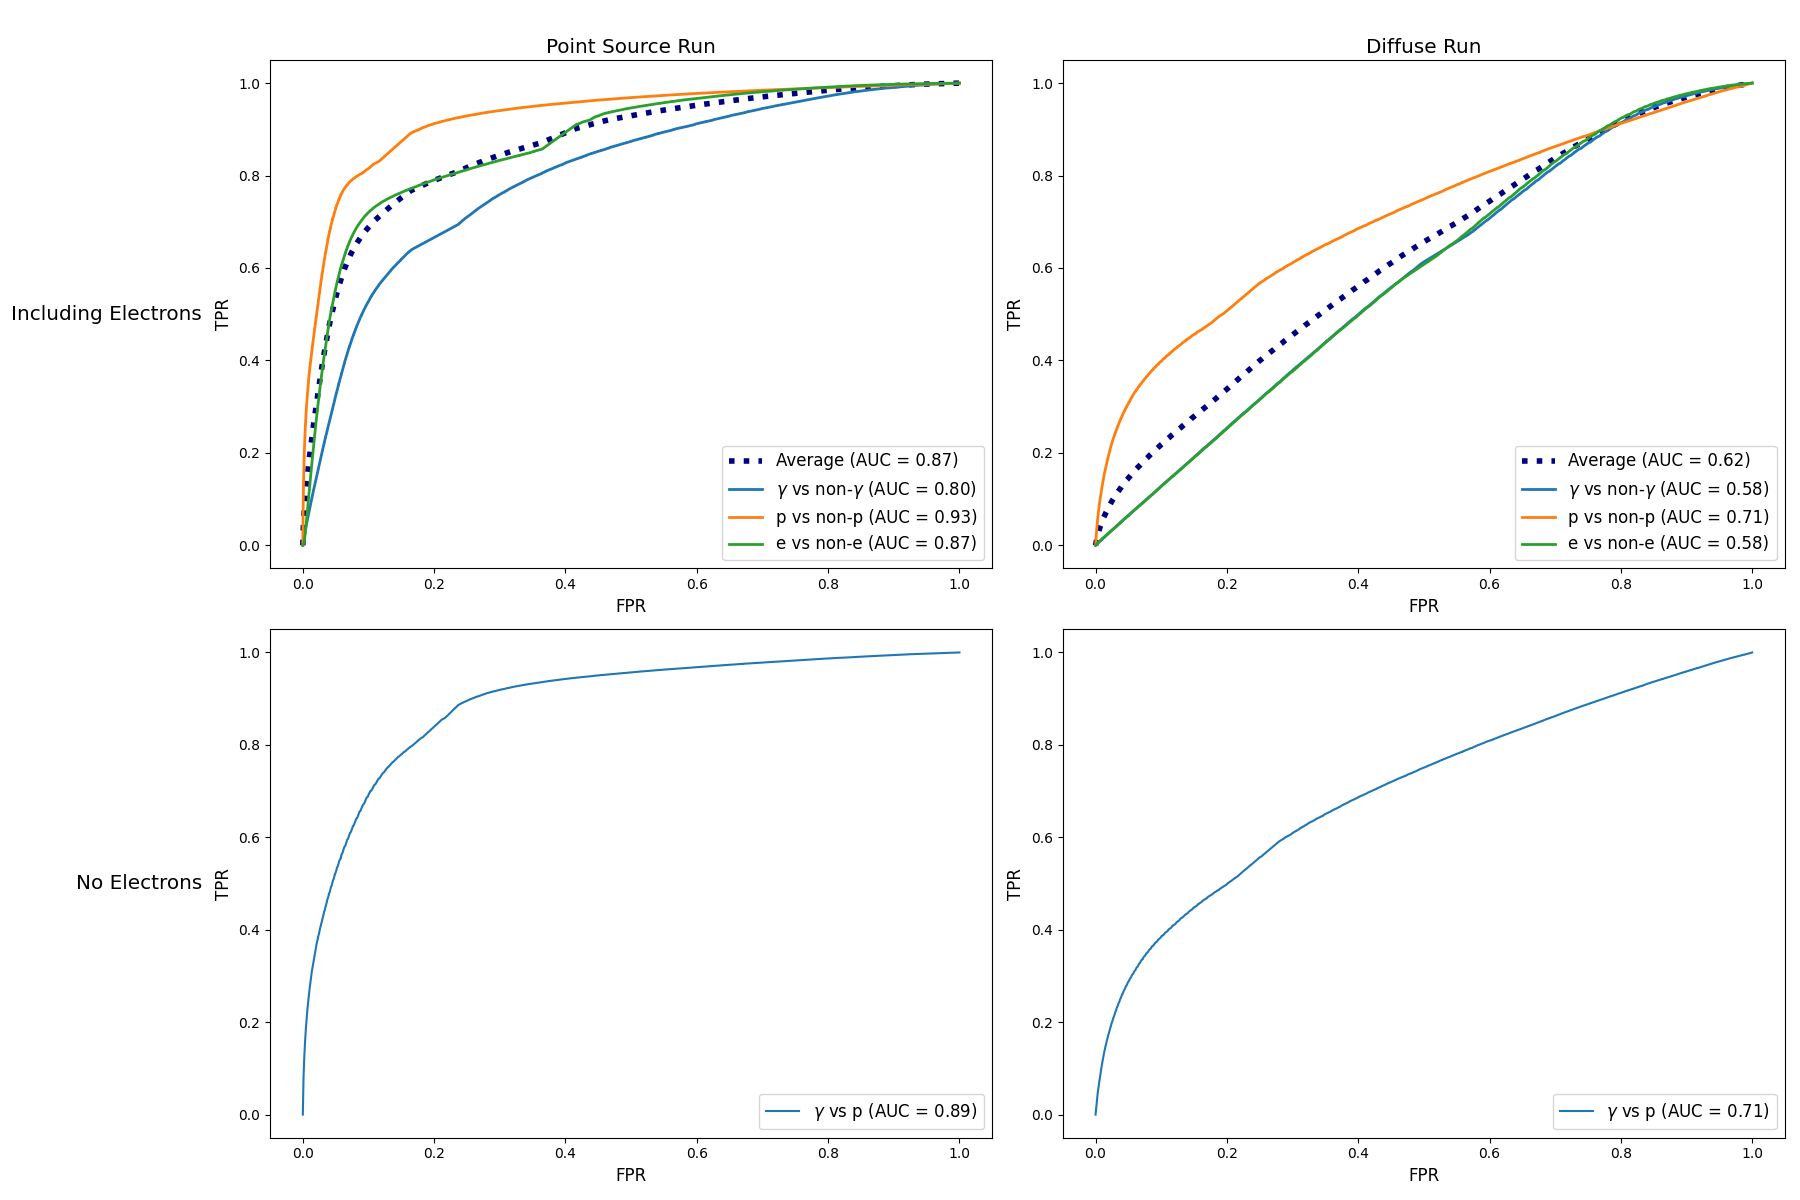
\includegraphics[width=1.0\columnwidth]{figures/rfplot.png}

        % note that in above figure file name, "sr_setup",
        % the file extension is missing. LaTeX is smart enough to find
        % apropriate one (i.e. pdf, png, etc.)
        % You can add this extention yourself as it seen below
        % both notations are correct but above has more flexibility
        %\includegraphics[width=1.0\columnwidth]{sr_setup.pdf}
        \caption{
                \label{fig:rfplot} % spaces are big no-no withing labels
                % things like fig: are optional in the label but it helps
                % to orient yourself when you have multiple figures,
                % equations and tables
                Point source and Diffuse RF test ROC curves with AUC values shown, showing the effect of inclusion of electrons.
        }
\end{figure}

These clearly show (expected) inferior performances of the RFs on these data, as well as clearly demonstrating that the presence of electrons in the data has a significant effect on the average AUC value. However given the issues with applying CNN-type methods to real data explored in the next chapter, it is likely these RFs would still outperform the ConvLSTM on real observations.

\section{Conclusions} \label{Conclusions}
We have investigated four methods of applying new deep learning methods to the task of classifying events for IACTs, finding that the use of timing information is an viable method of event discrimination against simulated hadronic air showers. Whilst not a full sensitivity analysis, our results demonstrate the value in including timing information in future CTA deep learning analyses. This became possible thanks to the significant technical innovation that has gone into the design of CHEC and other similar modern Cherenkov cameras. Our work also demonstrates that there is little prospect of CNN-based methods being used to filter out electron induced air showers, and so in future IACT deep learning studies (in the SST energy range) electrons should be treated as an irreducible background. That said, future IACT instruments (such as the CTA-affiliated Swartzchild-Couder Telescope with it's 12000 pixel camera \cite{psct}) may provide even more detailed images of EAS that might make electron event rejection feasible if used in combination with these techniques.

Another area of uncertainty related to this research is whether the representation of stereoscopic timing information in \textit{sim\_telarray} is sufficiently accurate to be used for these purposes. In the absence of multiple SSTs existing on site this is difficult to currently test, however we speculate that it might be possible to overcome such errors by simply adding offsets to the timing histograms based on telescope pointing and shower direction.

